%%%%%%%%%%%%%%%%%%%%%%%%%%%%%%%%%%%%%%%%%
% Programming/Coding Assignment
% LaTeX Template
%
% This template has been downloaded from:
% http://www.latextemplates.com
%
% Original author:
% Ted Pavlic (http://www.tedpavlic.com)
%
% Note:
% The \lipsum[#] commands throughout this template generate dummy text
% to fill the template out. These commands should all be removed when 
% writing assignment content.
%
% This template uses a Perl script as an example snippet of code, most other
% languages are also usable. Configure them in the "CODE INCLUSION 
% CONFIGURATION" section.
%
%%%%%%%%%%%%%%%%%%%%%%%%%%%%%%%%%%%%%%%%%

%----------------------------------------------------------------------------------------
%	PACKAGES AND OTHER DOCUMENT CONFIGURATIONS
%----------------------------------------------------------------------------------------

\documentclass[12pt]{article}
\usepackage{fix-cm} %for huge text

\usepackage{fancyhdr} % Required for custom headers
\usepackage{lastpage} % Required to determine the last page for the footer
\usepackage{extramarks} % Required for headers and footers
\usepackage[usenames,dvipsnames]{color} % Required for custom colors
\usepackage{graphicx} % Required to insert images
\usepackage{float}% For clipping images 
\usepackage{listings} % Required for insertion of code
\usepackage{courier} % Required for the courier font
\usepackage{lipsum} % Used for inserting dummy 'Lorem ipsum' text into the template
\usepackage{amsmath}% For nice mathematical formulas
\usepackage{amssymb} %for N, Z, R ...
\usepackage{subcaption}

% Margins
\topmargin=-0.45in
\evensidemargin=0in
\oddsidemargin=0in
\textwidth=6.5in
\textheight=9.0in
\headsep=0.25in

\linespread{1.1} % Line spacing

% Set up the header and footer
\pagestyle{fancy}
\lhead{\hmwkAuthorName} % Top left header
\chead{\hmwkClass} % Top center head
\rhead{\firstxmark} % Top right header
\lfoot{\lastxmark} % Bottom left footer
\cfoot{} % Bottom center footer
%\rfoot{Page\ \thepage\ of\ \protect\pageref{LastPage}} % Bottom right footer
\rfoot{\thepage} % Bottom right footer
\renewcommand\headrulewidth{0.4pt} % Size of the header rule
\renewcommand\footrulewidth{0.4pt} % Size of the footer rule

\setlength\parindent{0pt} % Removes all indentation from paragraphs
\newcommand{\comp}[1]{\textbf{\texttt {#1}}}% For writing computer terms
\newcommand{\important}{\textcolor{Red}{\textbf{Important: }}}
\newcommand{\hint}{\textcolor{MyBlue}{\textbf{Tip: }}}
%----------------------------------------------------------------------------------------
%	CODE INCLUSION CONFIGURATION
%----------------------------------------------------------------------------------------
%\renewcommand{\ttdefault}{pcr}
\definecolor{MyBlue}{rgb}{0.0,0.4,0.8} 
\definecolor{MyRed}{rgb}{1.0,0.3,0.3} 
\definecolor{MyYellow}{rgb}{1.0,0.7,0.07} % 
\definecolor{MyGray}{rgb}{0.9,0.9,0.9} % 
\definecolor{MyDarkGray}{rgb}{0.25,0.27, 0.32} % 
\definecolor{MyGreen}{rgb}{0.5,0.92, 0.95} % 
\definecolor{MyDarkGreen}{rgb}{0.0,0.4,0.0} % This is the color used for comments
\lstloadlanguages{C++} % Load Perl syntax for listings, for a list of other languages supported see: ftp://ftp.tex.ac.uk/tex-archive/macros/latex/contrib/listings/listings.pdf

\lstset{language=C++, % Use Perl in this example
        frame=single, % Single frame around code
        backgroundcolor=\color{MyDarkGray}, % set backgroundcolor
        xleftmargin=0.5cm, frame=tlbr, framesep=5pt, framerule=0pt,
        basicstyle=\linespread{1.1}\small\ttfamily\color{MyGray}, % Use small true type font
        keywordstyle=[1]\color{MyYellow}, % Perl functions bold and blue
        keywordstyle=[2]\color{MyYellow}\bf, % 
        keywordstyle=[3]\color{Red}\bf, % Custom functions underlined and blue
        otherkeywords = {;,(,),\,,::, [, ]},
    	morekeywords = [3]{;},
    	morekeywords = [2]{::, (,),\,, [,]},
        identifierstyle=, % Nothing special about identifiers                                         
        commentstyle=\usefont{T1}{pcr}{m}{sl}\color{MyGreen}\small, % Comments small dark green courier font
        moredelim=**[is][\color{MyYellow}]{@}{@},% make color for text between @text@
        stringstyle=\color{MyRed}, % Strings are purple
        showstringspaces=false, % Don't put marks in string spaces
        tabsize=4, % 5 spaces per tab
        %
        % Put standard Perl functions not included in the default language here
        morekeywords={rand},
        %
        % Put Perl function parameters here
        morekeywords=[2]{on, off, interp},
        %
        % Put user defined functions here
        morekeywords=[3]{test},
       	%
        morecomment=[l][\color{Green}]{...}, % Line continuation (...) like blue comment
        numbers=left, % Line numbers on left
        firstnumber=1, % Line numbers start with line 1
        numberstyle=\tiny\color{MyDarkGray}, % Line numbers are blue and small
        stepnumber=1 % Line numbers go in steps of 5
}

% Creates a new command to include a perl script, the first parameter is the filename of the script (without .pl), the second parameter is the caption
\newcommand{\perlscript}[2]{
\begin{itemize}
\item[]\lstinputlisting[caption=#2,label=#1]{#1.pl}
\end{itemize}
}

%----------------------------------------------------------------------------------------
%	DOCUMENT STRUCTURE COMMANDS
%	Skip this unless you know what you're doing
%----------------------------------------------------------------------------------------

% Header and footer for when a page split occurs within a problem environment
\newcommand{\enterProblemHeader}[1]{
%\nobreak\extramarks{#1}{#1 continued on next page\ldots}\nobreak
%\nobreak\extramarks{#1 (continued)}{#1 continued on next page\ldots}\nobreak
\nobreak\extramarks{#1}{}\nobreak
}


% Header and footer for when a page split occurs between problem environments
\newcommand{\exitProblemHeader}[1]{
%\nobreak\extramarks{#1 (continued)}{#1 continued on next page\ldots}\nobreak
%\nobreak\extramarks{#1}{}\nobreak
}

%\setcounter{secnumdepth}{0} % Removes default section numbers
\newcounter{homeworkProblemCounter} % Creates a counter to keep track of the number of problems

\newcommand{\homeworkProblemName}{}
\newenvironment{homeworkProblem}[1][Problem \arabic{homeworkProblemCounter}]{ % Makes a new environment called homeworkProblem which takes 1 argument (custom name) but the default is "Problem #"
\stepcounter{homeworkProblemCounter} % Increase counter for number of problems
\renewcommand{\homeworkProblemName}{#1} % Assign \homeworkProblemName the name of the problem
\section{\homeworkProblemName} % Make a section in the document with the custom problem count
\setlength\parindent{18pt}
\enterProblemHeader{\homeworkProblemName} % Header and footer within the environment
}{
%\exitProblemHeader{\homeworkProblemName} % Header and footer after the environment
}

\newcommand{\problemAnswer}[1]{ % Defines the problem answer command with the content as the only argument
\noindent\framebox[\columnwidth][c]{\begin{minipage}{0.98\columnwidth}#1\end{minipage}} % Makes the box around the problem answer and puts the content inside
}

\newcommand{\homeworkSectionName}{}
\newenvironment{homeworkSection}[1]{ % New environment for sections within homework problems, takes 1 argument - the name of the section
%\renewcommand{\homeworkSectionName}{#1} % Assign \homeworkSectionName to the name of the section from the environment argument
\subsection{\homeworkSectionName} % Make a subsection with the custom name of the subsection
\setlength\parindent{18pt}
\enterProblemHeader{\homeworkProblemName\ [\homeworkSectionName]} % Header and footer within the environment
}{
\enterProblemHeader{\homeworkProblemName} % Header and footer after the environment
}

%----------------------------------------------------------------------------------------
%	NAME AND CLASS SECTION
%----------------------------------------------------------------------------------------

\newcommand{\hmwkTitle}{What\ I\ can\ and\ what\ I\ cannot\ do\ with\ PCA} % Assignment title
\newcommand{\hmwkDueDate}{Monday,\ January\ 1,\ 2012} % Due date
\newcommand{\hmwkClass}{PCA\ Manual} % Course/class
\newcommand{\hmwkClassTime}{10:30am} % Class/lecture time
\newcommand{\hmwkClassInstructor}{Jones} % Teacher/lecturer
\newcommand{\hmwkAuthorName}{Anna Sinelnikova} % Your name

%----------------------------------------------------------------------------------------
%	TITLE PAGE
%----------------------------------------------------------------------------------------

\newcommand*{\titleAT}{\begingroup % Create the command for including the title page in the document
\newlength{\drop} % Command for generating a specific amount of whitespace
\drop=0.1\textheight % Define the command as 10% of the total text height

\rule{\textwidth}{1pt}\par % Thick horizontal line
\vspace{2pt}\vspace{-\baselineskip} % Whitespace between lines
\rule{\textwidth}{0.4pt}\par % Thin horizontal line

\vspace{\drop} % Whitespace between the top lines and title
\centering % Center all text
\textcolor{MyBlue}{ % Red font color
{{\fontsize{50}{70}\selectfont PCA Manual}}\\[0.5\baselineskip] % Title line 1
{\Large OR}\\[0.75\baselineskip] % Title line 2
{\Huge How to Succeed in Rescaling of Polymers}} % Title line 3

\vspace{0.25\drop} % Whitespace between the title and short horizontal line
\rule{0.3\textwidth}{0.4pt}\par % Short horizontal line under the title
\vspace{\drop} % Whitespace between the thin horizontal line and the author name

{\Large \textsc\hmwkAuthorName}\par % Author name

%\vfill % Whitespace between the author name and publisher text
%{\large \textcolor{Red}{\plogo}}\\[0.5\baselineskip] % Publisher logo
\begin{figure}[H]
\centering

\includegraphics[width=0.82\linewidth]{scaling2.eps}
\end{figure}
\vspace{-4cm}
%{\large \textsc{Uppsala University, 2016}}\par % Publisher

\vspace*{\drop} % Whitespace under the publisher text

\rule{\textwidth}{0.4pt}\par % Thin horizontal line
\vspace{2pt}\vspace{-\baselineskip} % Whitespace between lines
\rule{\textwidth}{1pt}\par % Thick horizontal line

\endgroup}

%----------------------------------------------------------------------------------------

\begin{document}

\thispagestyle{empty} % Removes page numbers
\titleAT
%----------------------------------------------------------------------------------------
%	TABLE OF CONTENTS
%----------------------------------------------------------------------------------------

%\setcounter{tocdepth}{1} % Uncomment this line if you don't want subsections listed in the ToC

\newpage
\tableofcontents
\newpage
\section*{Introduction} 
PCA project consists from:
\begin{enumerate}
\item Independent PCA library in \comp{C++11}.
\item Three example applications in \comp{C++11}.
\item \comp{MATLAB} script for plotting one or several chains which are obteined during scaling procedure.
\item Another \comp{MATLAB} script for making movies of scaling process, where one scaling step is one frame.
\item Small script for \comp {GNUplot} for plotting the figure of dependency of total angle on scaling step.
\item Some chains of proteins from Protein Data Bank (PDB) for quick start.
\item Library documentation for developers, which was generated automatically in ``doxygen".
\end{enumerate}
The program unfortunately does not have any graphical user interface. So you can work with it only from the terminal. However the only thing you should know is how to change the directory there. All the rest you can do with your favourite file managers and text editor.
%----------------------------------------------------------------------------------------
% ALGORITHM
%----------------------------------------------------------------------------------------

\begin{homeworkProblem}[Algorithm]\label{sec:theory}
\subsection{Theory}
Let us assume we have a chain of solid rigid segments. All we need to describe this kind of system is coordinates of all sites of the chain.
\begin{figure}
	\centering
	\vskip -0cm 
	\begin{subfigure}{0.45\linewidth}
  		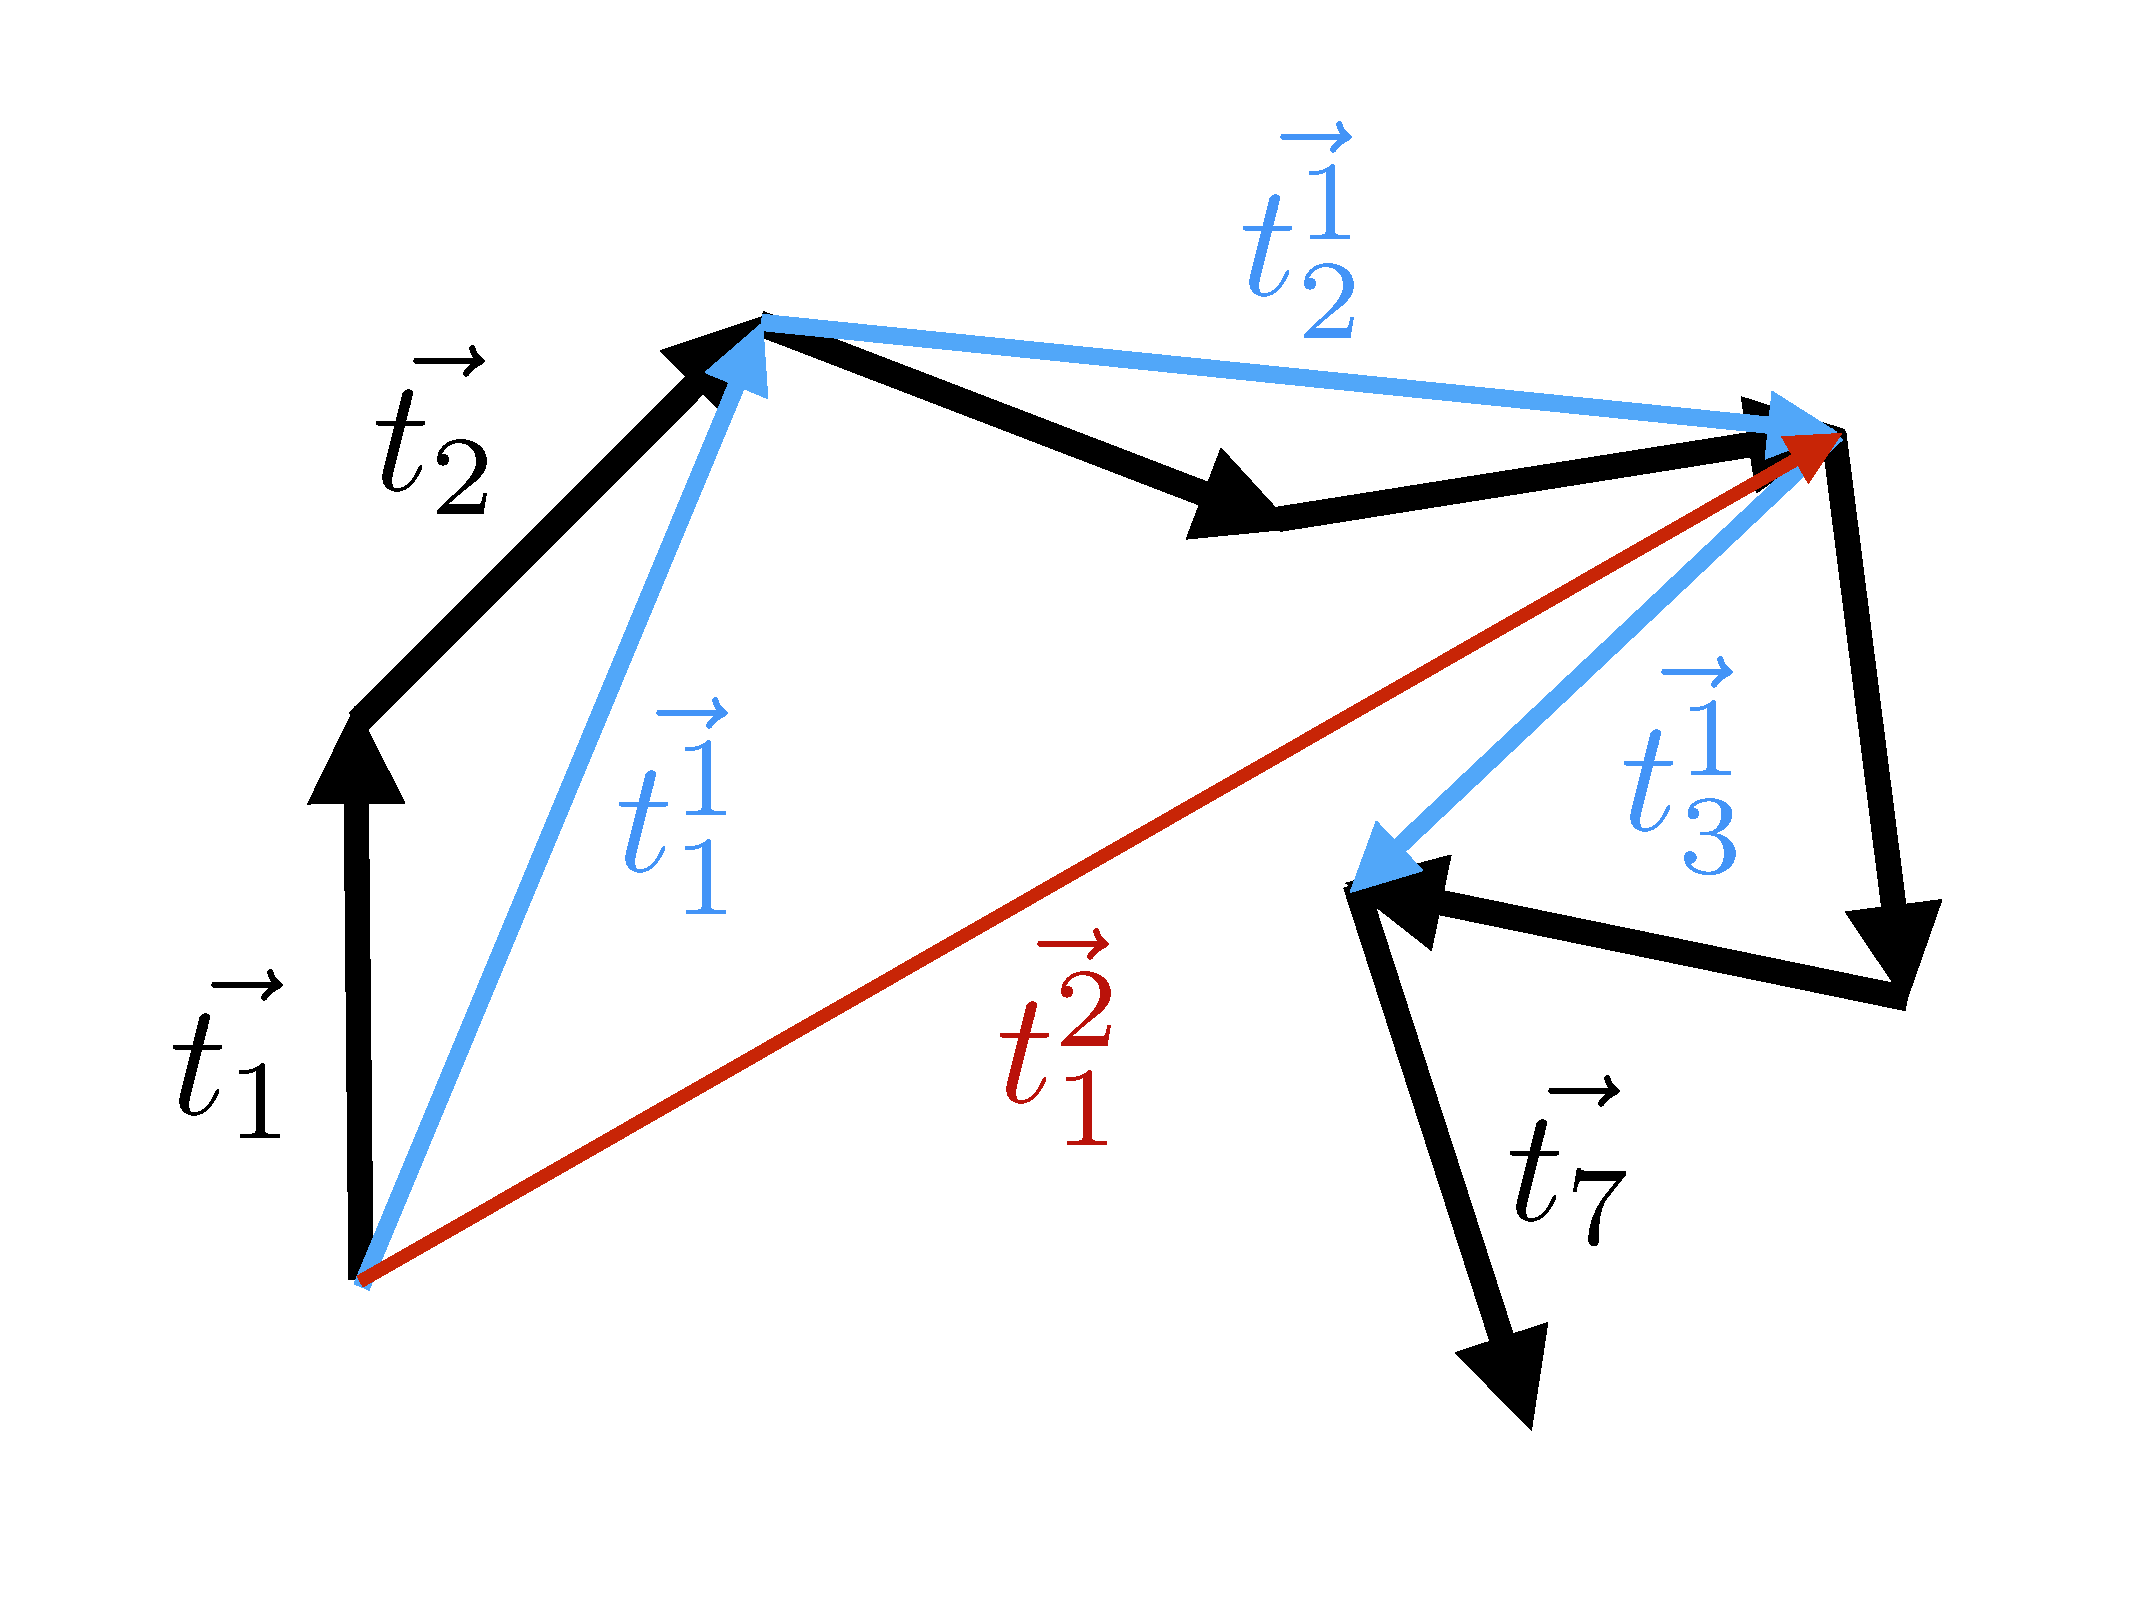
\includegraphics[width=1.0\linewidth]{figure-1.pdf}
  		\caption{$s = 2$.}
  	\end{subfigure}
  	\begin{subfigure}{0.45\linewidth}
  		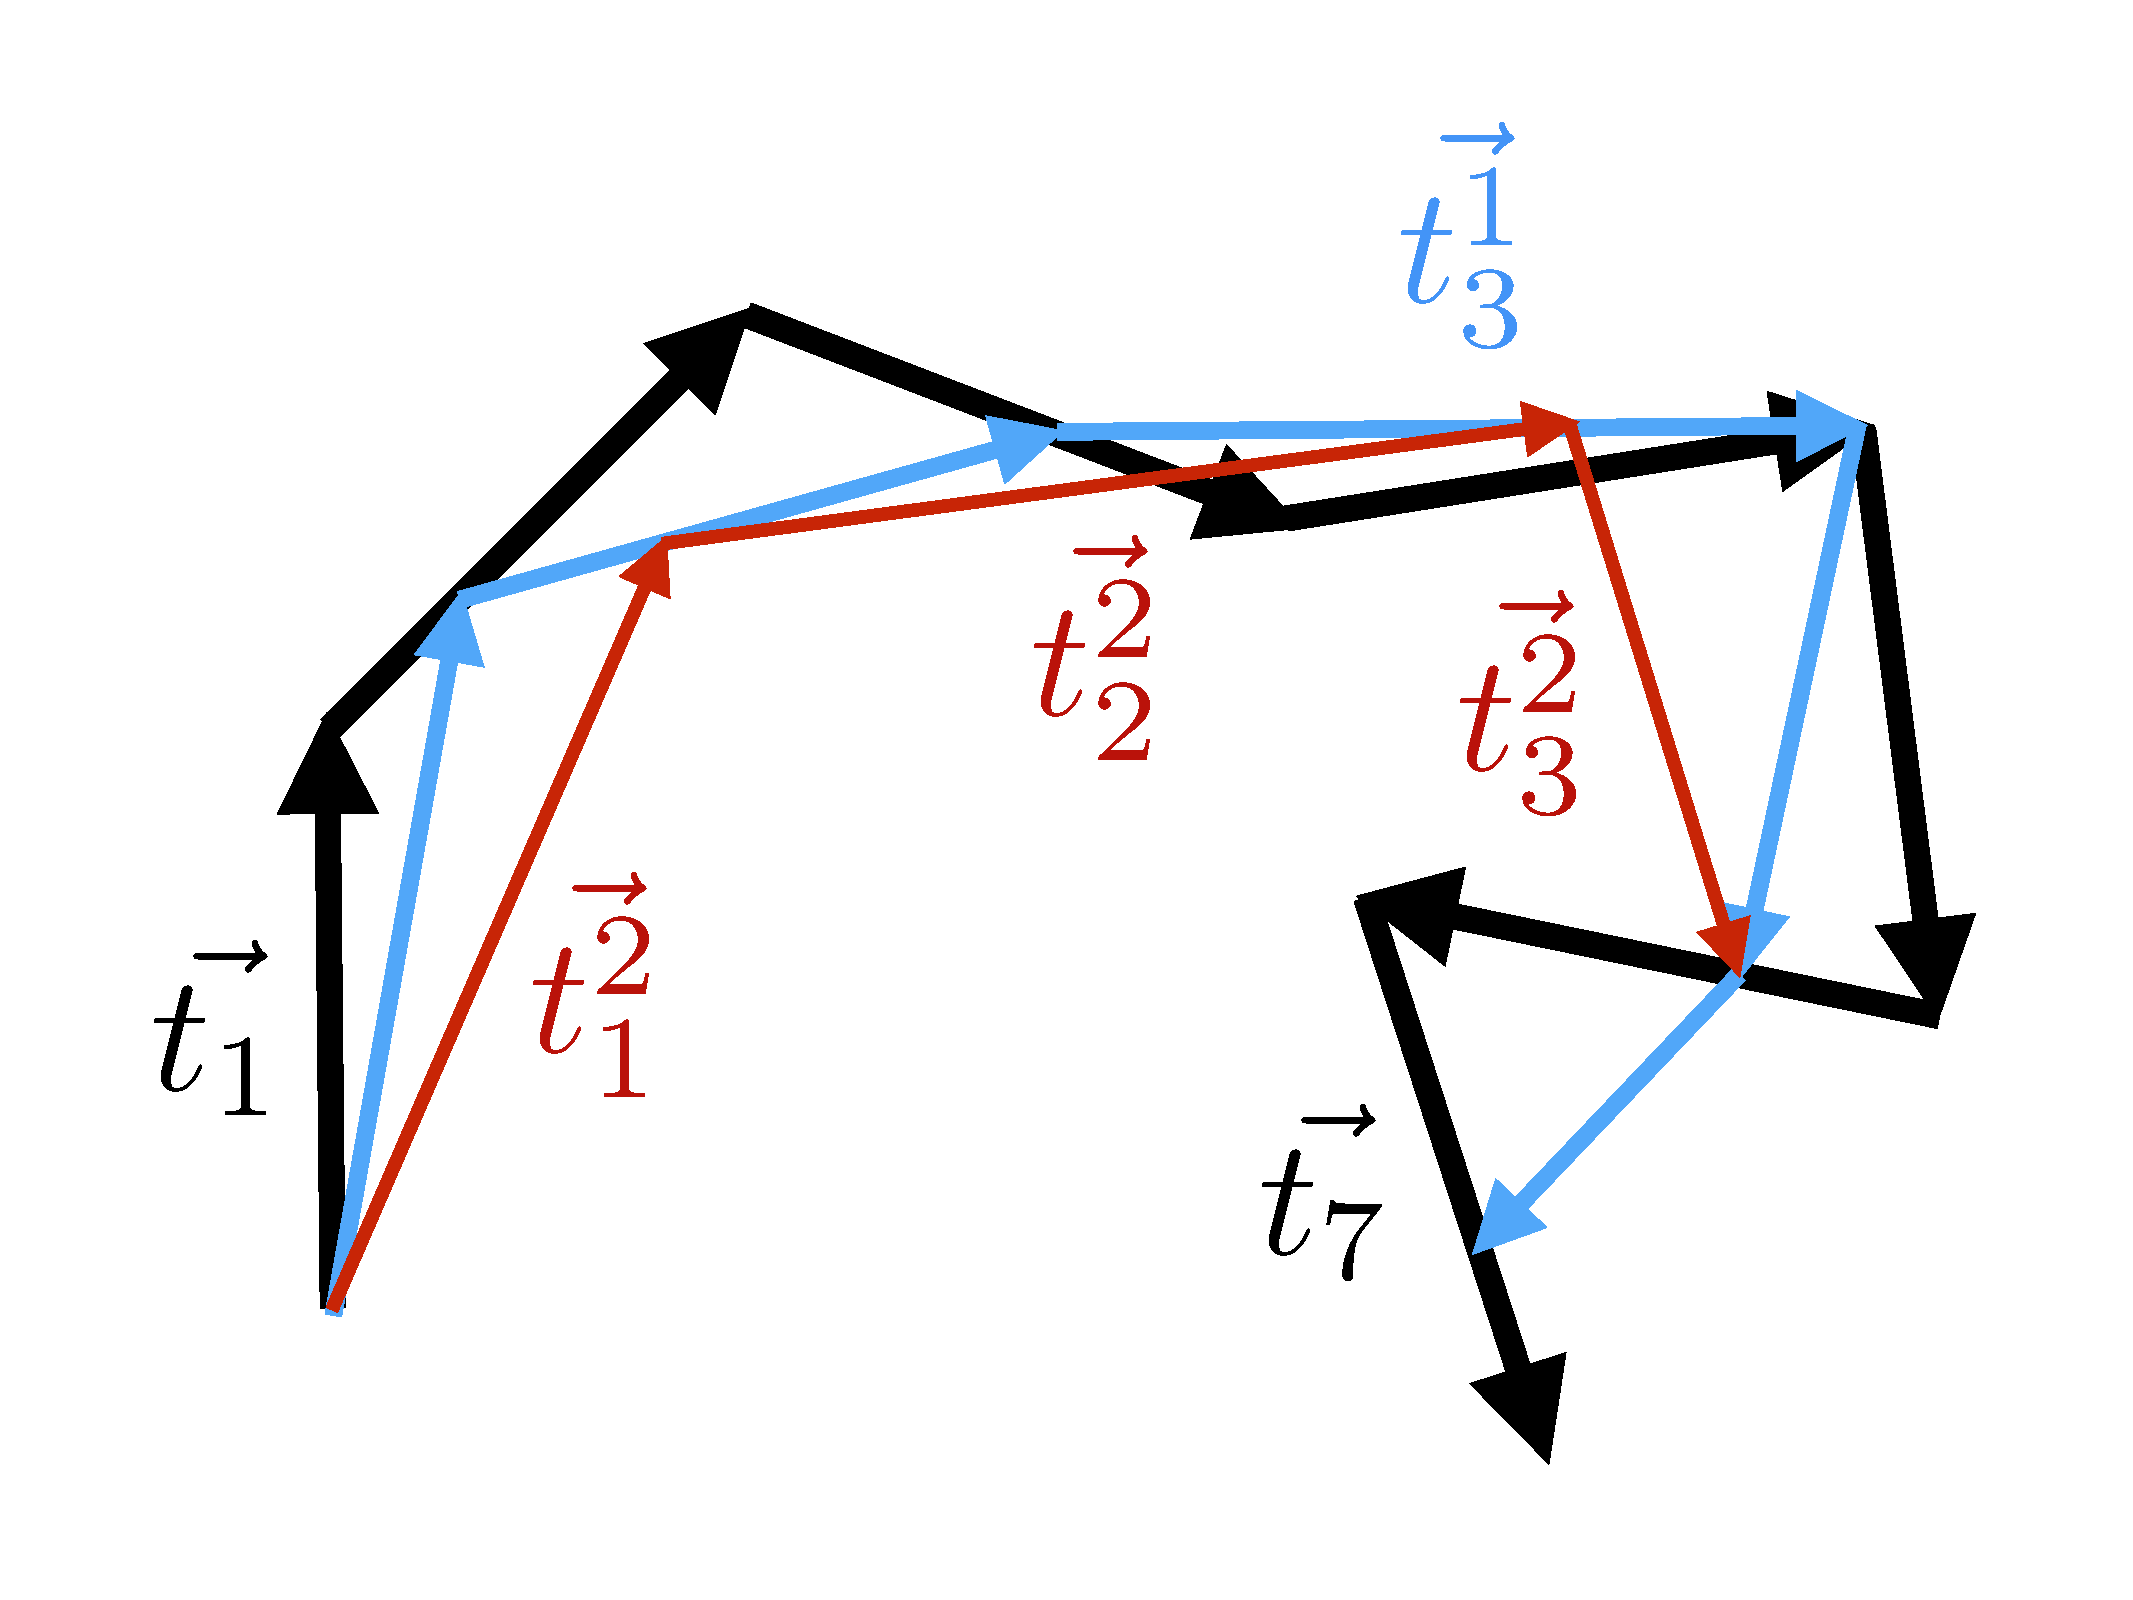
\includegraphics[width=1.0\linewidth]{figure-2.pdf}
  		\caption{$s = \frac{4}{3}$.}
  	\end{subfigure}
  	\caption{Illustration of two first steps of scaling procedure for various scaling parameter $s$. }
	\label{fig:theoreticalScaling}
\end{figure}
Now we want to do some kind or rescaling of the system. The simpliest idea is to connect every second site with new link. It is illustrated in Figure \ref{fig:theoreticalScaling} (a) with blue lines.
If $\vec{t_1}\,,\vec{t_2}\,,...$ are vectors along links of original chain, then after the first step of rescaling procedure we get $\vec{t_1^1}\,,\vec{t_2^1}\,,...$. This new blue chain also can be rescaled in the same way, thus we have the second step of the procedure: red line in Figure \ref{fig:theoreticalScaling} (a) $\vec{t_1^2}\,,\vec{t_2^2}\,,...$. For long enough chains we can have more than 3 iteration steps. However, the length of the original chain reduces quite quick, by $2^p$, where $p$ is number of iteration step.

Let $s$ denote number of old monomers in a new one. Then  in the previous case $s=2$. What if we take not integer $s$? This situation is presented in Figure \ref{fig:theoreticalScaling} (b). We do quite similar to the previous case thing, but instead of connecting two old links in a new one, we connect four thirds. More strictly for the first iteration step:

\begin{gather*}
\vec{t_1^1} = \vec{t_1} + \frac{1}{3}\vec{t_2}\\
\vec{t_2^1} = \frac{2}{3}\vec{t_2} + \frac{2}{3}\vec{t_3}\\
\vec{t_3^1} = \frac{1}{3}\vec{t_3} + \vec{t_4}
\end{gather*}

For the second iteration step we do the same but instead of the original chain we take the chain we got from the previous step.

\subsection{General algorithm}
Let us consider the general algorithm for any $s\in(1,+\infty)$, 

We can express $s$ as a rational fraction:
\begin{equation}
s = I+\frac{n}{d}\,,\;\;{\rm where}\;\;\; n\in \mathbb{N};\;\;I,\,d \in \mathbb{N}\backslash 0
\label{eq:s}
\end{equation}

Despite that the idea of that algorithm is not complicated, it is not possible to write it mathematically in a short way (like for the previous case), because of complicated indexation during scaling procedure. So let's look at the working algorithm instead, which is performed by function \comp{scaling} from class \comp{PolymerScaling}. This function is the core of the program, all other functions from the same class call \comp{scaling} finally.

The flowchart of the algorithm is presented in Figure \ref{fig:flowchart}. There we used together with (\ref{eq:s}) this expansion of scaling parameter:
\begin{equation}
s = {\rm intS} +{\rm fracS} 
\end{equation}

``k\%d" means that you should take the integer part of quotient, according C notation.

There are three cases in the algorithm. They are schematicaly shown in Figure \ref{fig:flowchart_branch}, where black chain is the old one, and blue is new. The right branch (Figure \ref{fig:branch3}) is the situation when new link starts from some old site. It means that some old site concisest with new one. Two other cases describe the opposite situation: new site divides old link into two parts. The difference between left branch and the middle one can be easily seen  in figures \ref{fig:branch2} and \ref{fig:branch3}.

\begin{figure}[t]
	\centering
	\vskip -0cm 
  	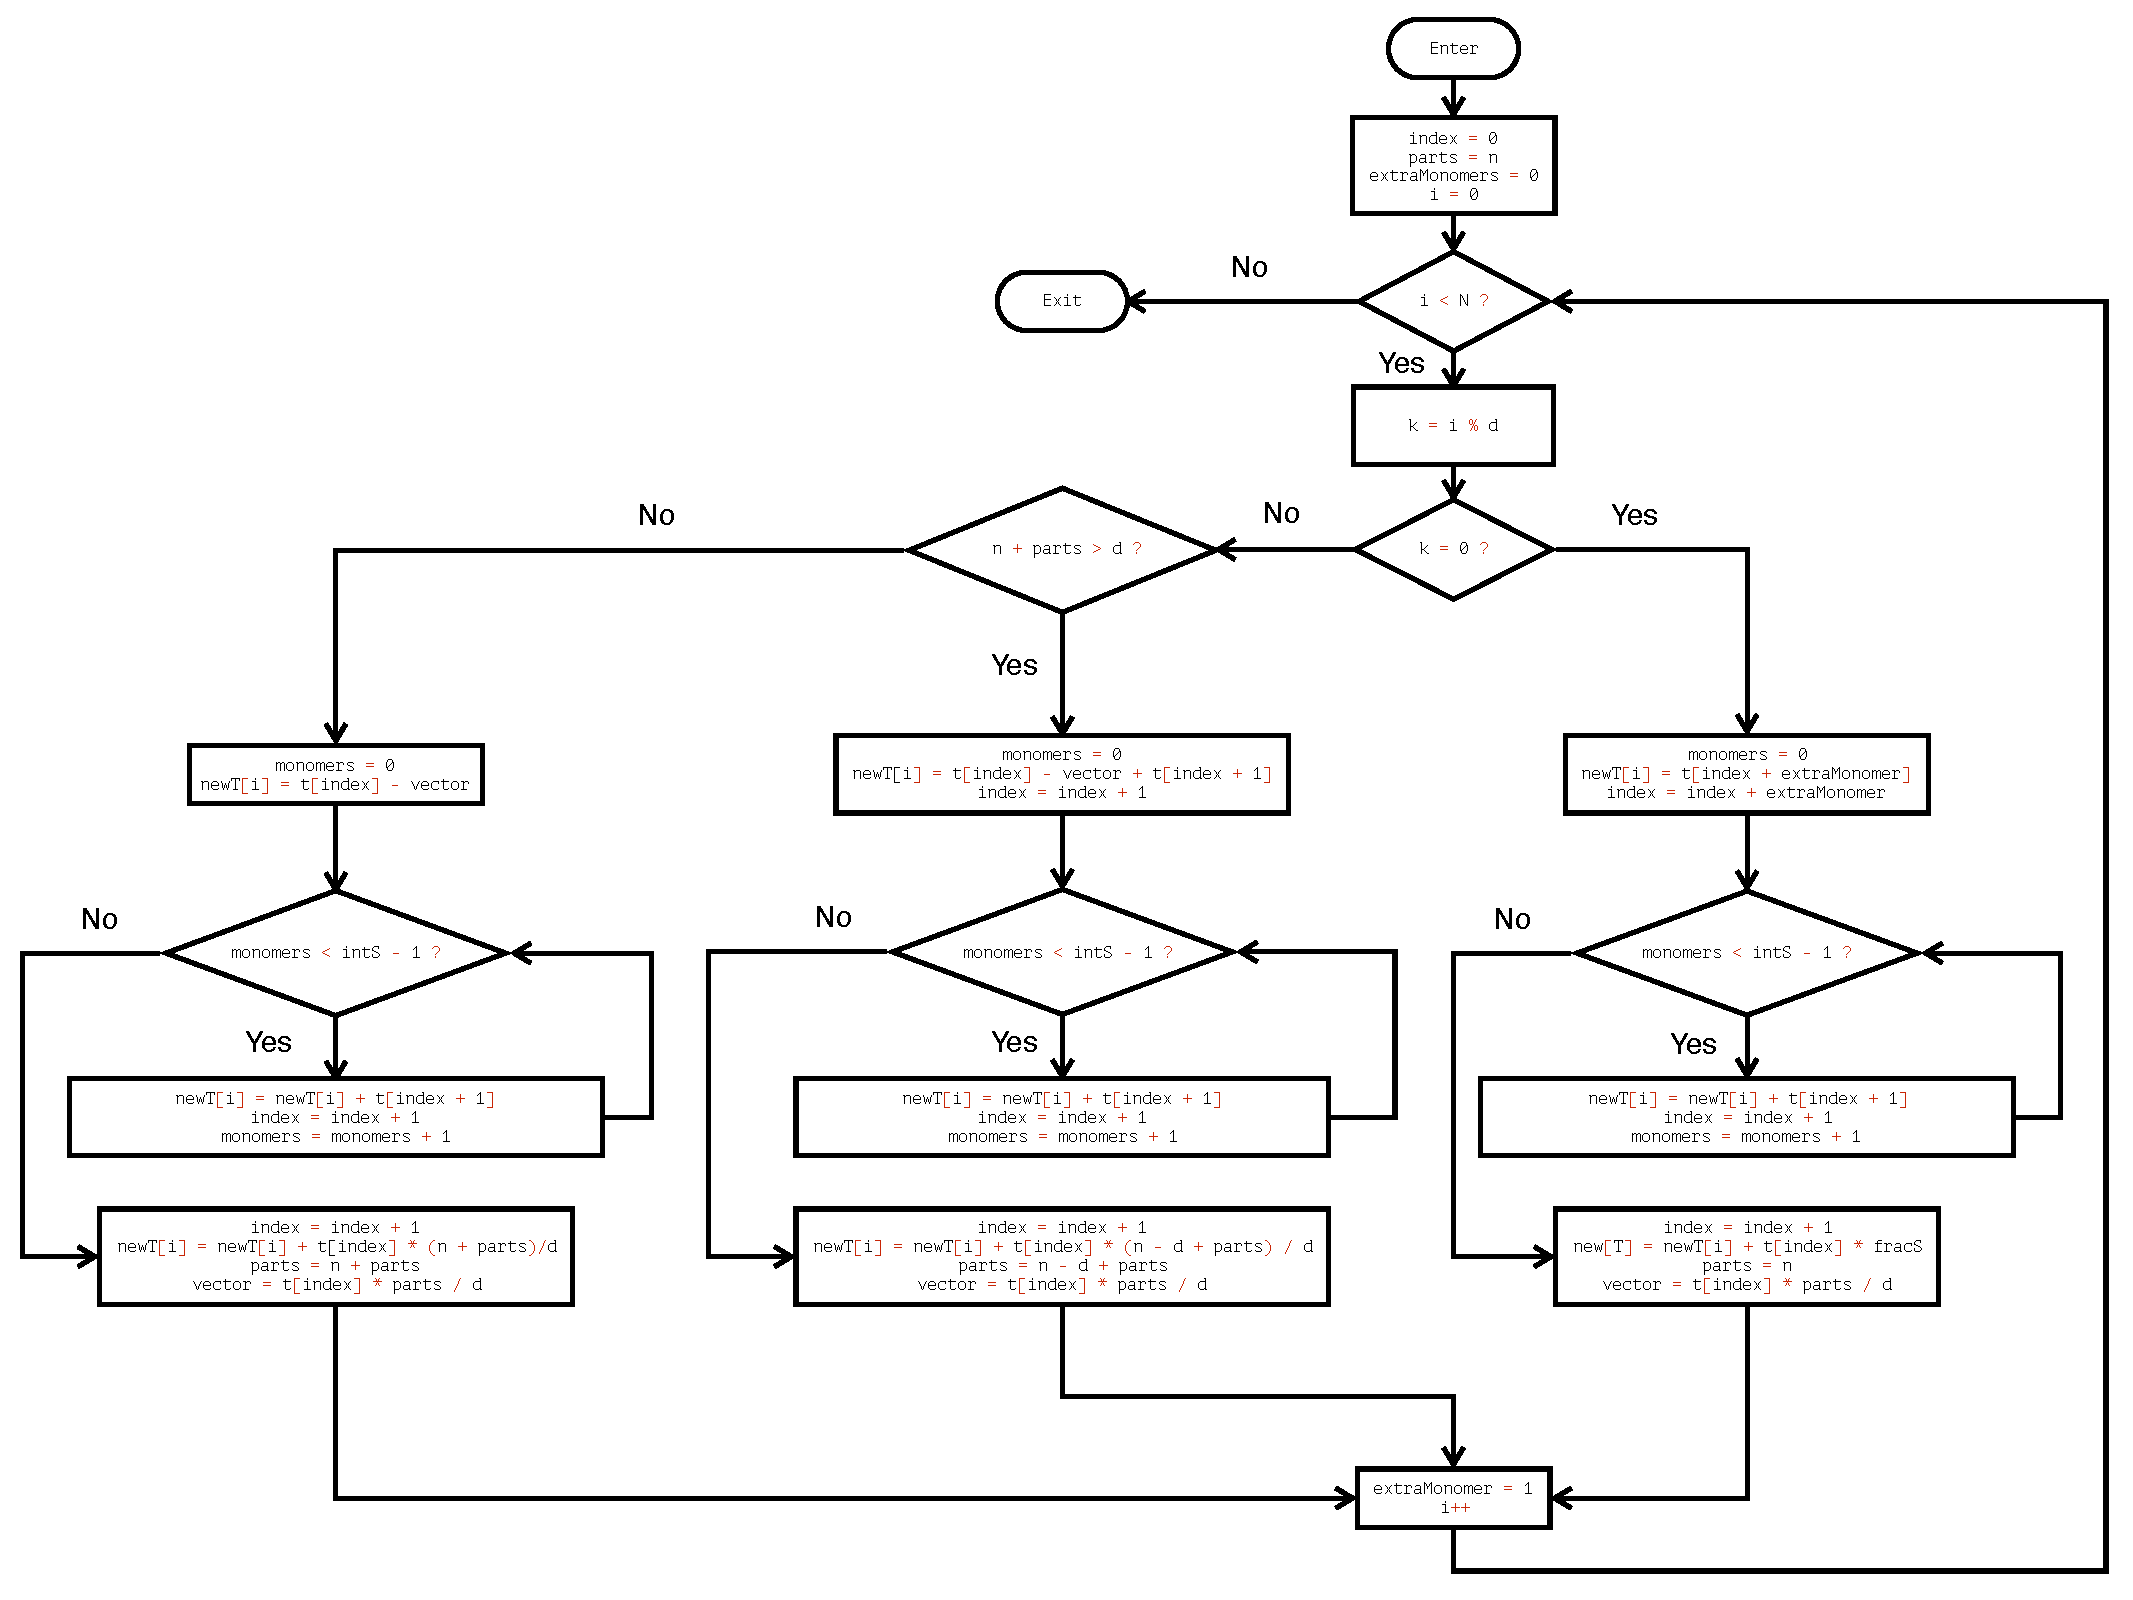
\includegraphics[width=1.0\linewidth]{Flowchart.pdf}
  	\caption{The flowchart of function \comp{PolymerScaling::scaling(...)}}
	\label{fig:flowchart}
\end{figure}

\begin{figure}
	\centering
	\vskip -0cm 
	\begin{subfigure}{0.3\linewidth}
  		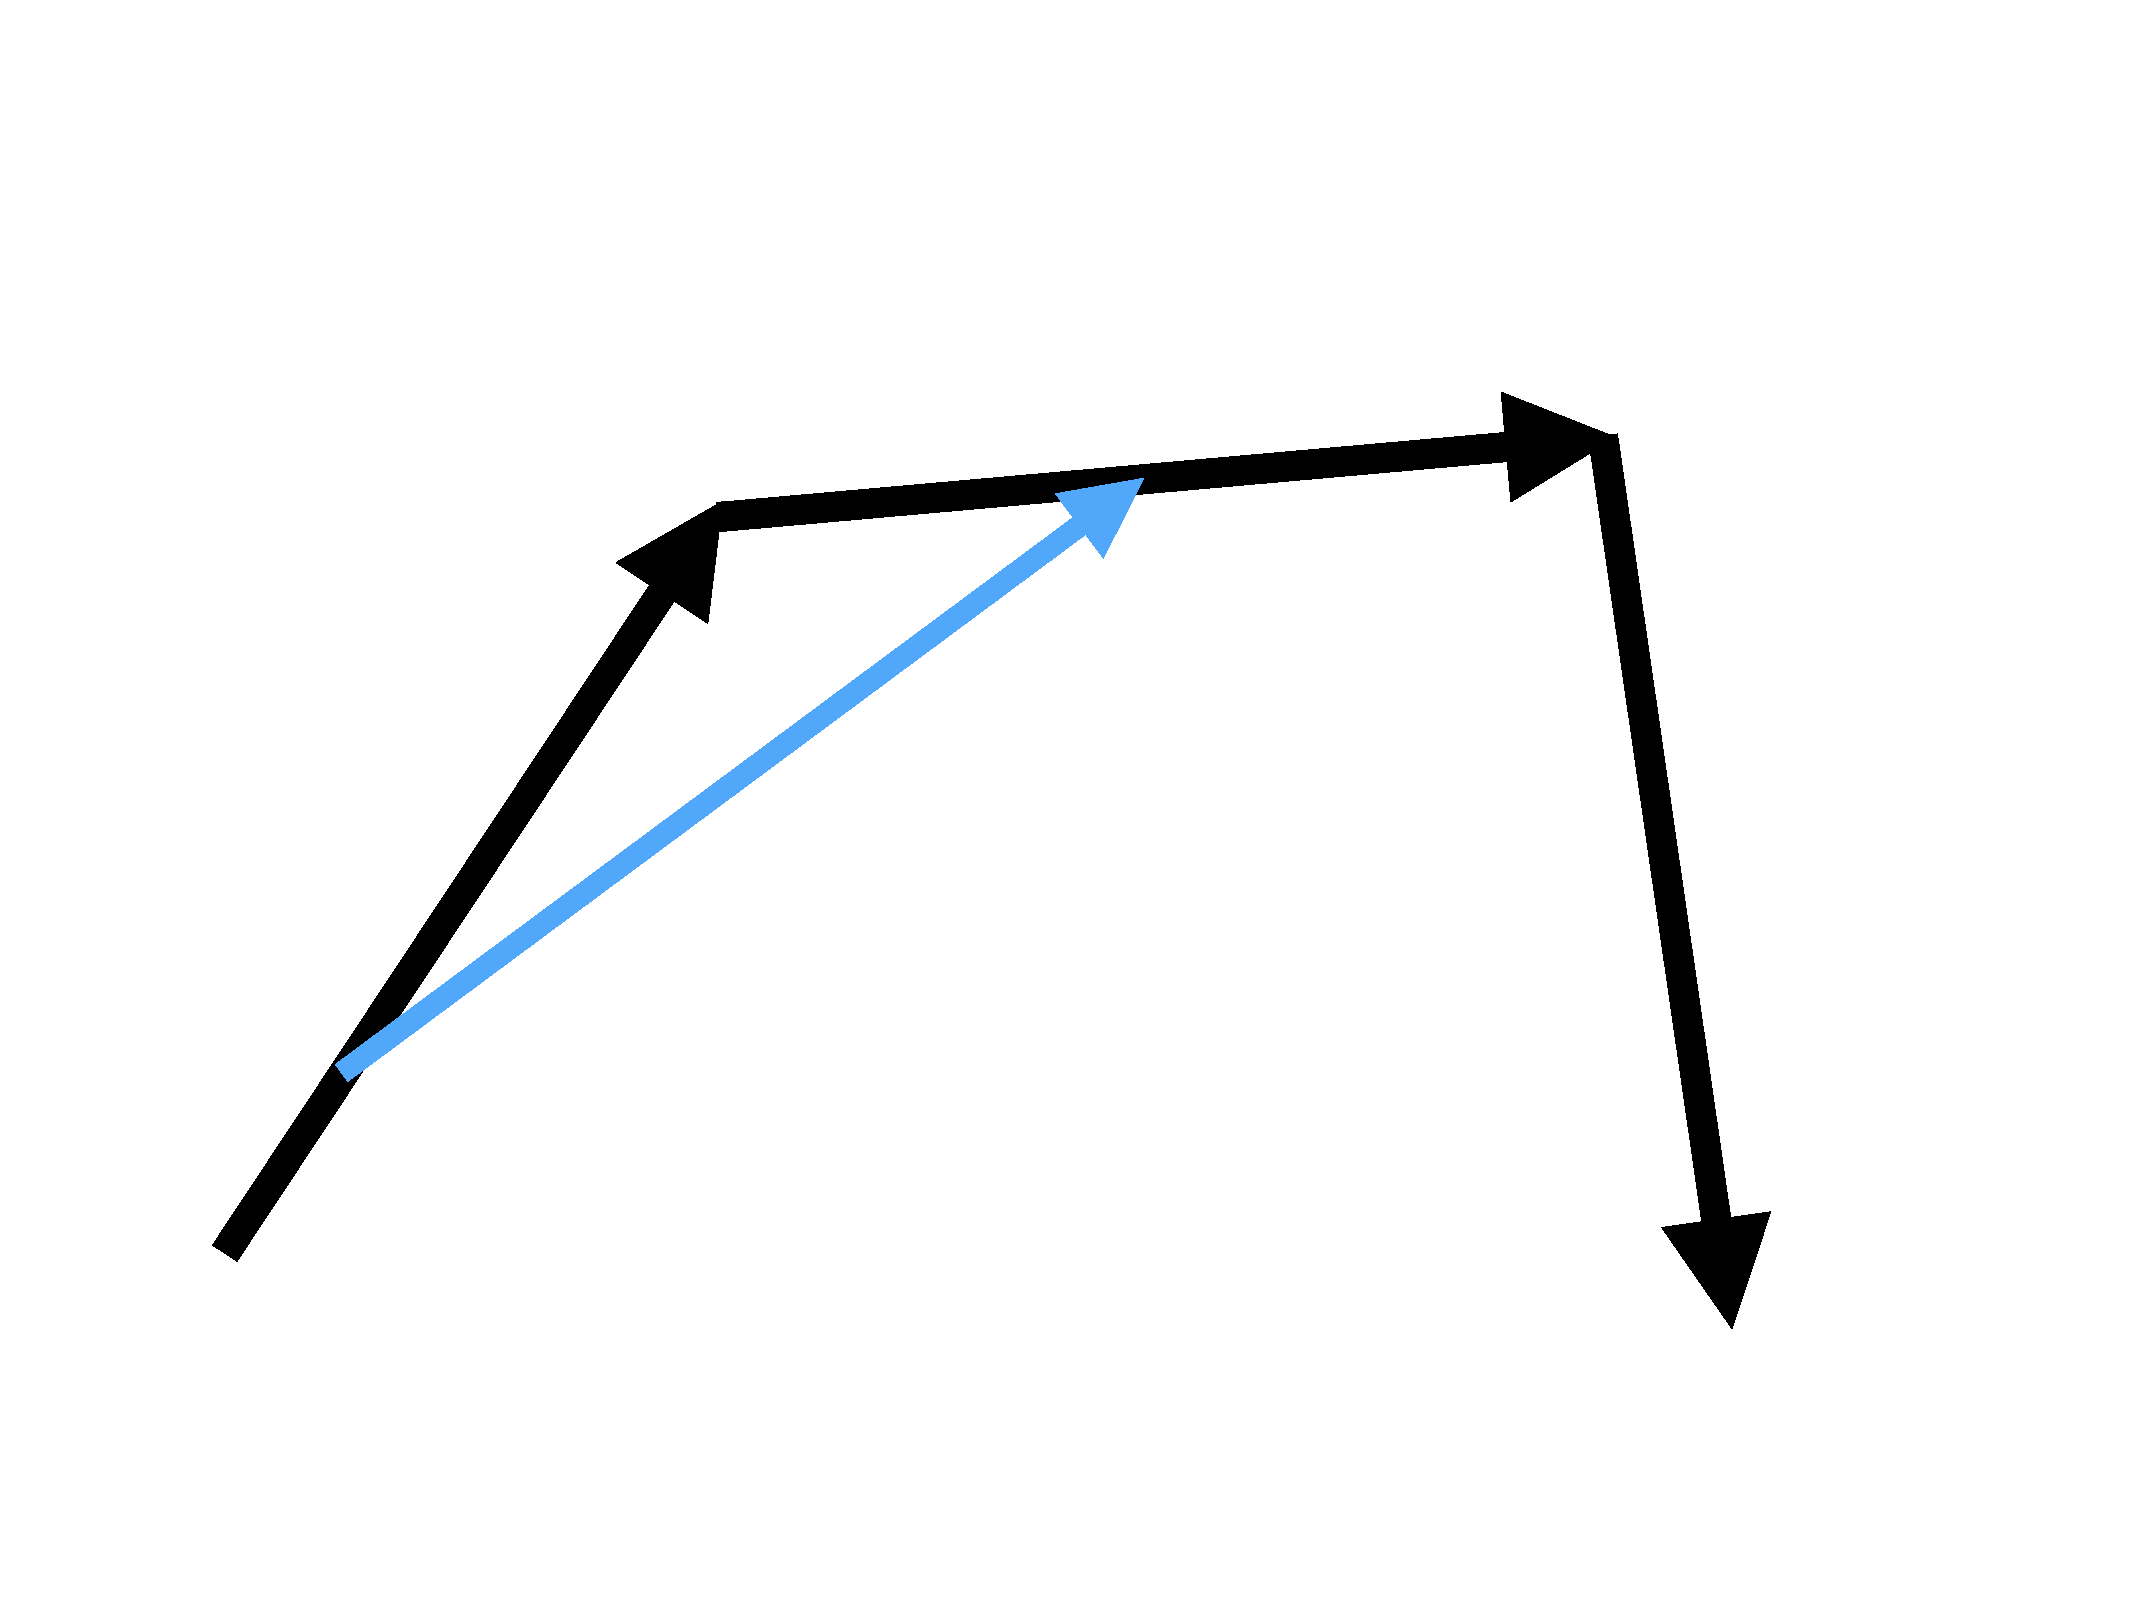
\includegraphics[width=1.0\linewidth]{Flowchart_branch1.pdf}
  		\caption{branch 1}
  		\label{fig:branch1}
  	\end{subfigure}
  	\begin{subfigure}{0.3\linewidth}
  		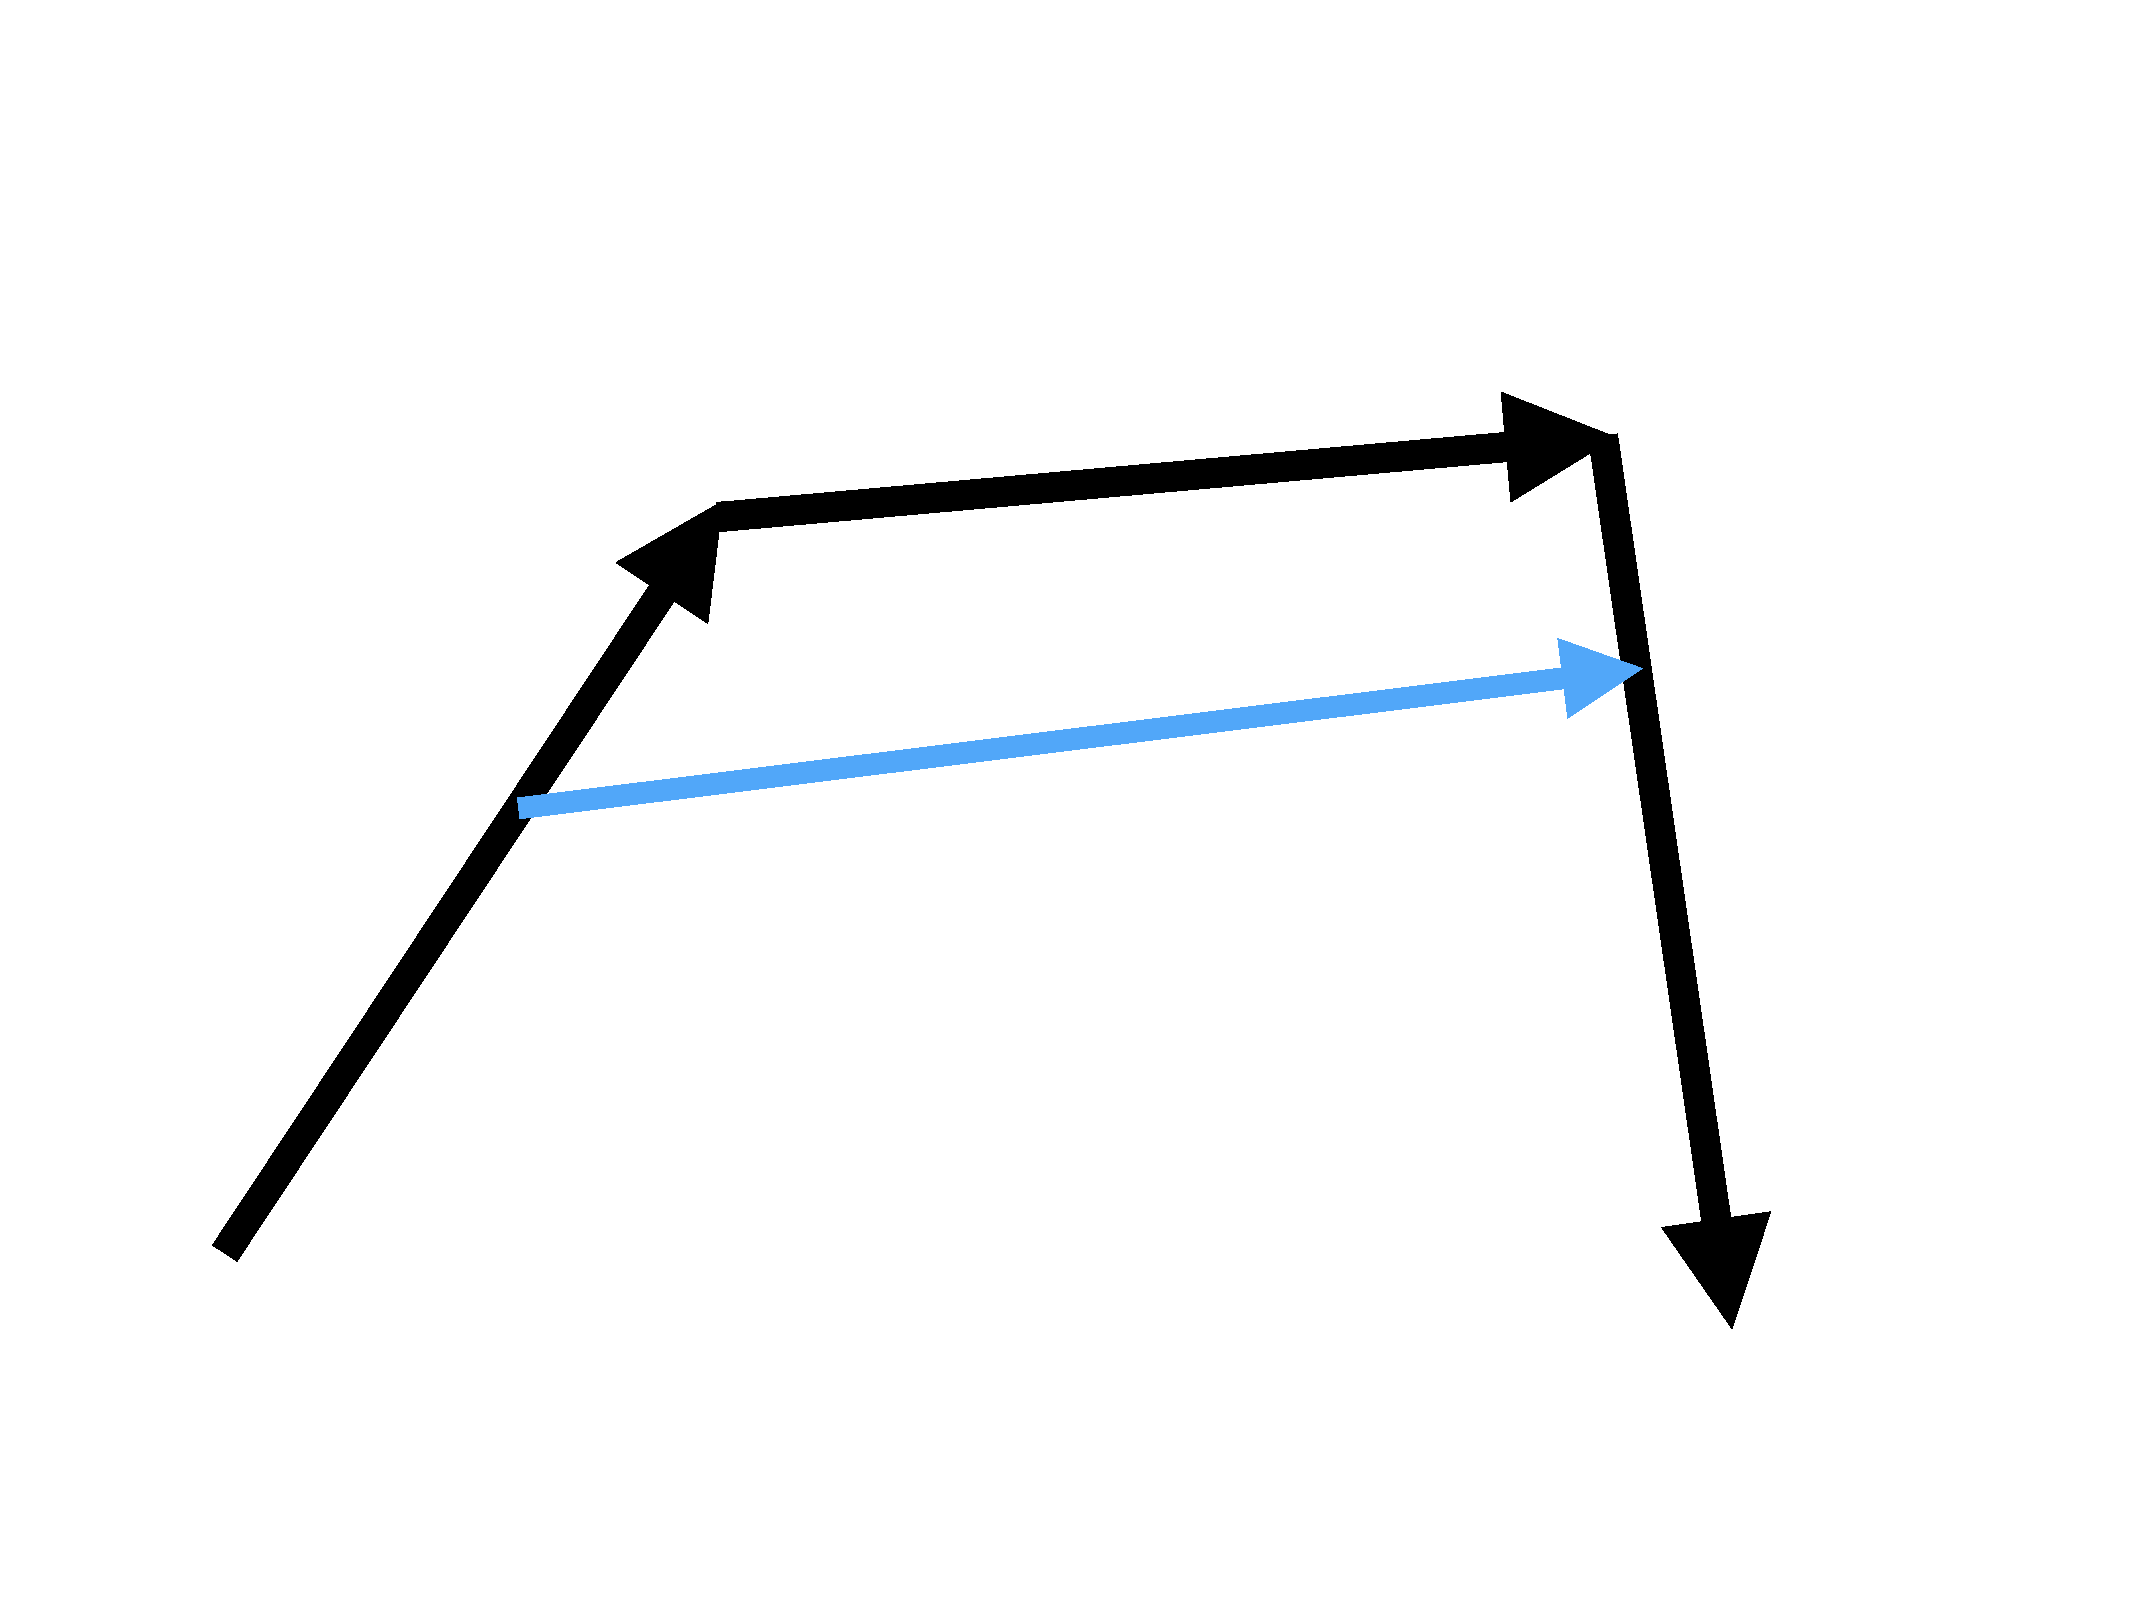
\includegraphics[width=1.0\linewidth]{Flowchart_branch2.pdf}
  		\caption{branch 2}
  		\label{fig:branch2}
  	\end{subfigure}
  	\begin{subfigure}{0.3\linewidth}
  		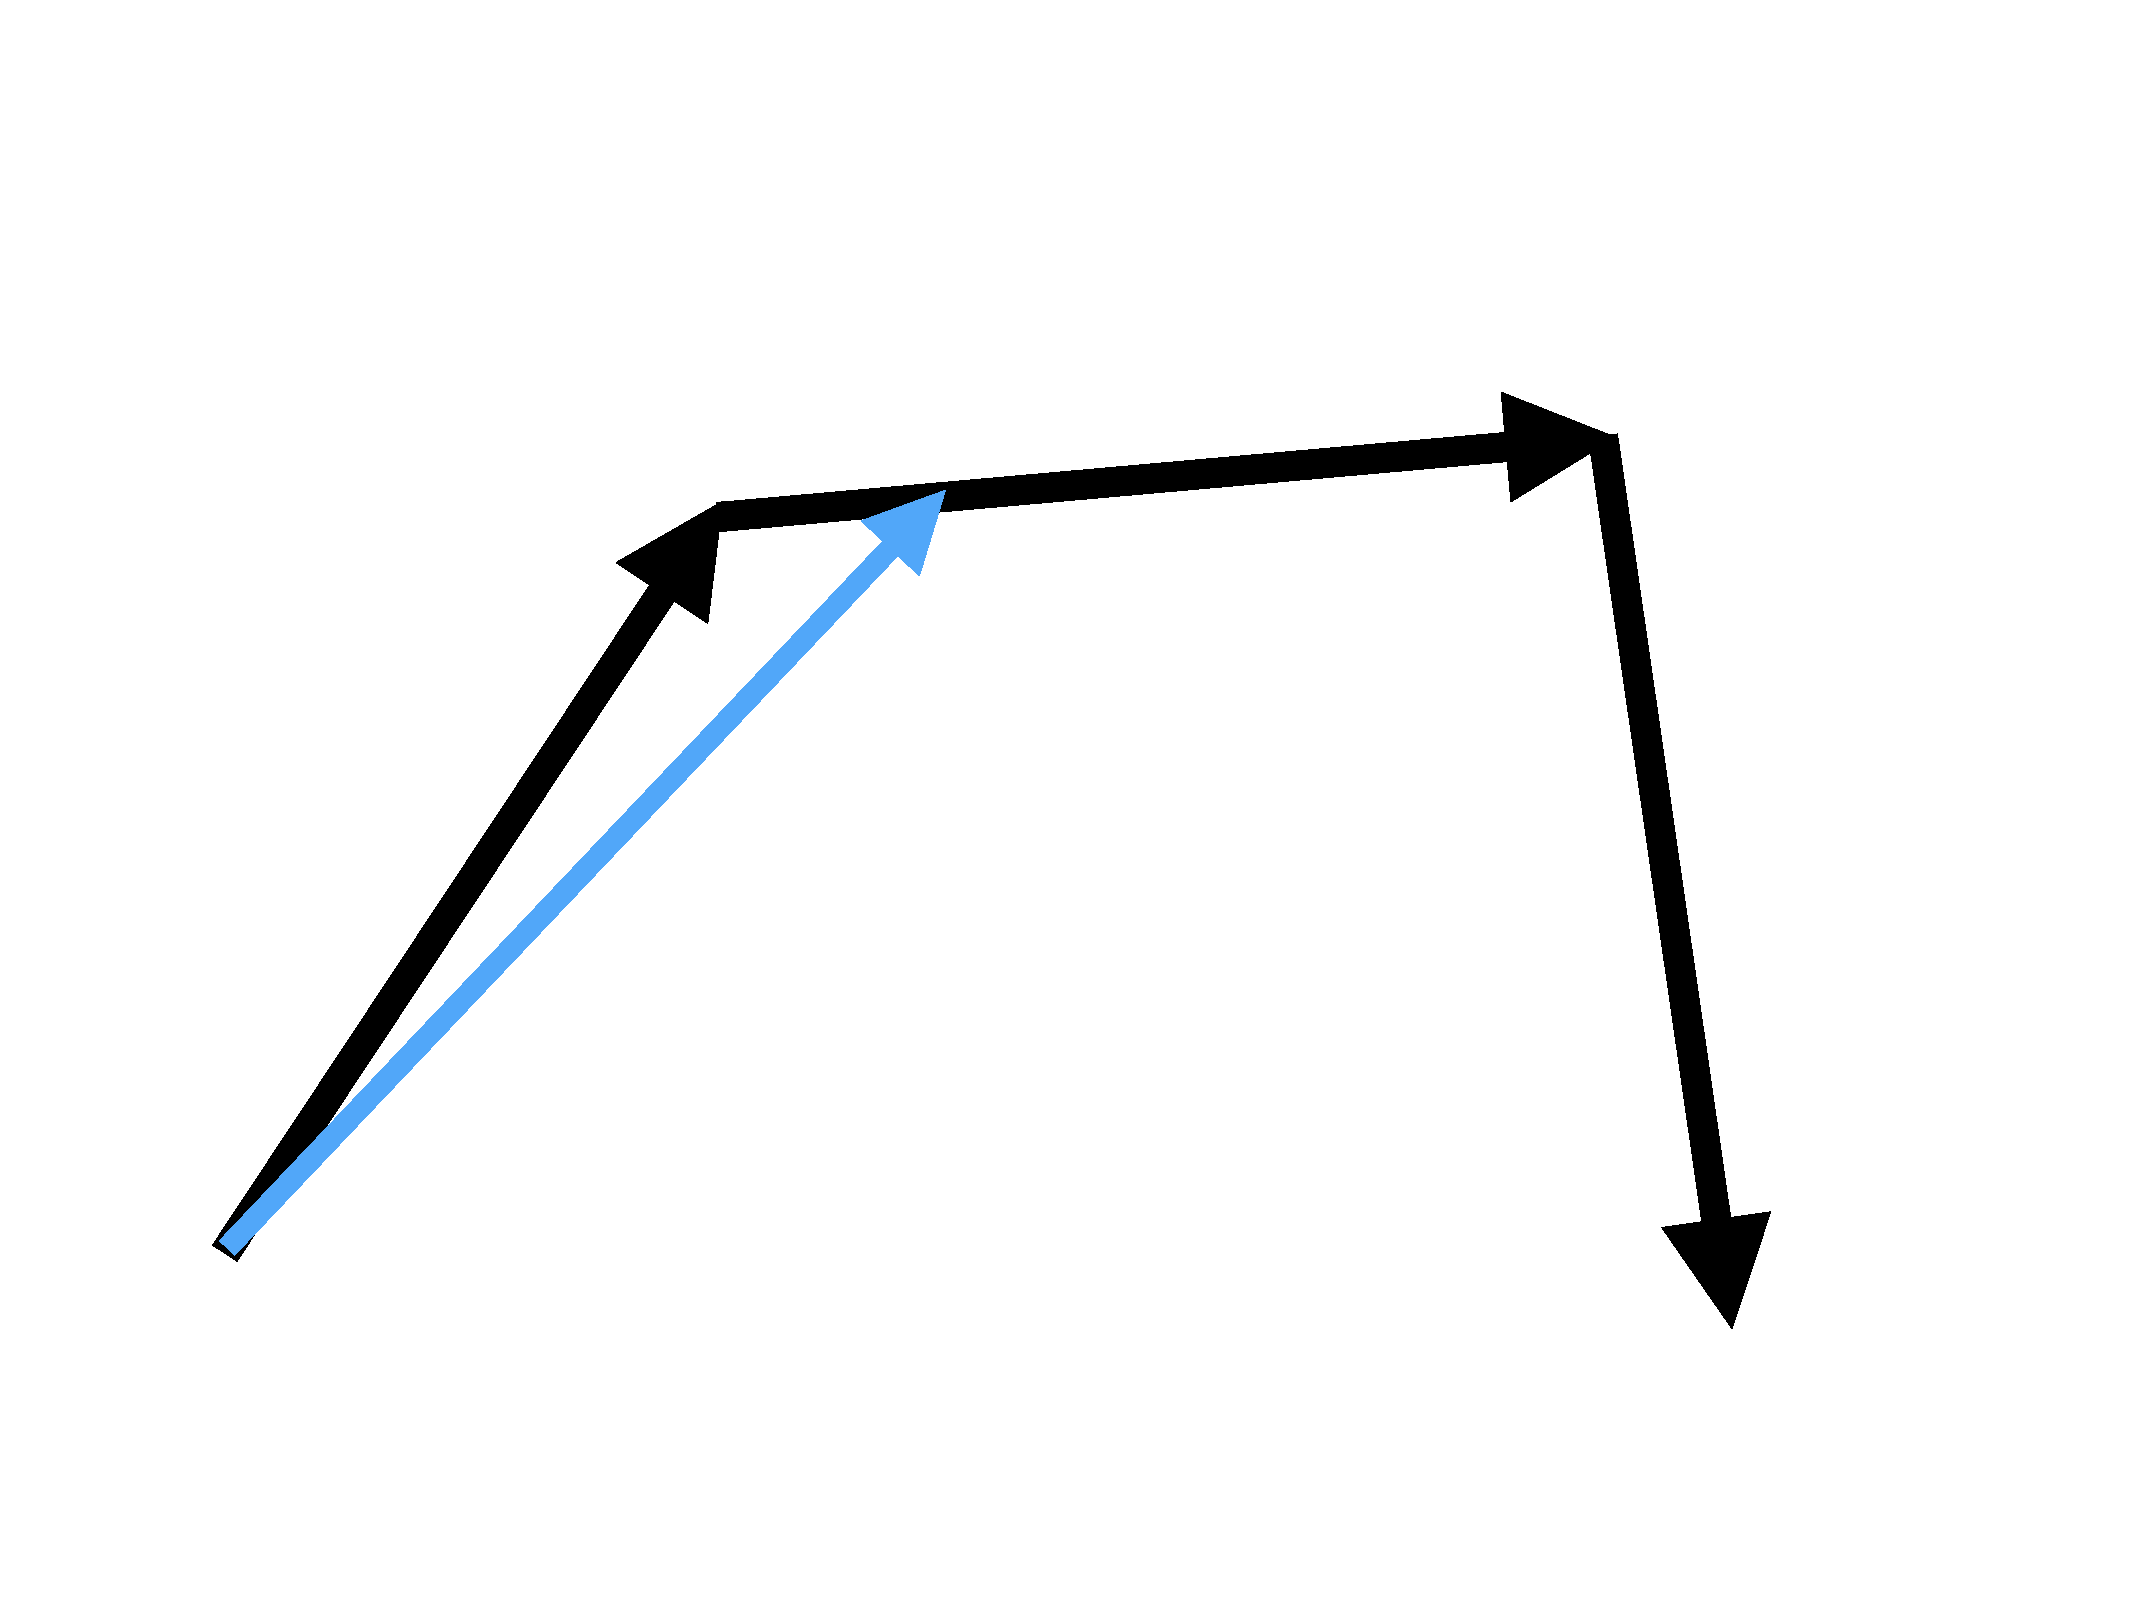
\includegraphics[width=1.0\linewidth]{Flowchart_branch3.pdf}
  		\caption{branch 3}
  		\label{fig:branch3}
  	\end{subfigure}
  	\caption{to flowchart}
	\label{fig:flowchart_branch}
\end{figure}

\end{homeworkProblem}
%----------------------------------------------------------------------------------------
% QUICK START
%----------------------------------------------------------------------------------------

\begin{homeworkProblem}[Quick Start]\label{sec:classPolymer}
Here is the instruction how one can quick run the program. The program does not have graphical interface, so all the work should be done from the terminal.
\subsection{Compilation the library}
First of all download PCA project to your computer from https://github.com/Anny-Moon/PCA. You can do it manually on the website or you can use \comp{git}:
\begin{lstlisting}
@$@ git clone https://github.com/Anny-Moon/PCA
\end{lstlisting}
The next step is to compile the PCA library on your computer (you are required to have \comp{gcc} compiler). Go to folder \comp{/PCA\_lib} in the main folder with project and do \comp{make}:
\begin{lstlisting}
@$@ cd PCA/PCA_lib
@PCA/PCA_lib$@ make
\end{lstlisting}
The compiler will show you which files it handled. And this line will show that library was successfully built:
\begin{lstlisting}
Generating static library... libpca.a
\end{lstlisting}
Now we want to make the library accessible from any folder on you computer. It will allow you to create applications and do not care about paths. Go back to root folder and start initialization session:
\begin{lstlisting}
@PCA/PCA_lib$@ cd ../
@PCA$@ source init_session.sh
\end{lstlisting}
\important initialization session should be done every time you start new terminal.


\subsection{Applications}
There are three things you can do:
\begin{enumerate}
\item \comp{scaling}: Scaling procedure without calculating any observables.
\item \comp{totalAngle}: Scaling procedure with calculating total angle for fixed parameter $k$ (see eq. \ref{eq:totalAngle}). If you have several chains in your file (see sec. \ref{sec:inputFile}) then it will calculate average total angle and error (see sec. \ref{sec:observableVSscalingStepWithStatistics}).
\item \comp{various\_k}: Scaling procedure with calculating total angle for broad range of $k$. If you have several chains in your  then it will calculate average total angle and error.
\end{enumerate}

Copy application you want to use somewhere on your computer. Then go to this folder and run make:
\begin{lstlisting}
@myApplication$@ make
\end{lstlisting}
Since you see this:
\begin{lstlisting}
Generating executable file.. pca
\end{lstlisting}
you are ready to start calculations.

Choose which polymer from folder \comp{data} in the project's root you want to analyze and pass the name as the first argument for the program like this:
\begin{lstlisting}
@PCA$@ ./pca 5dn7
\end{lstlisting}
It will run function \comp{observableVSscalingStep} for observable \comp{TotalAngle} for chain 5dn7 with writing all possible side files (see sec. \ref{sec:observableVSscalingStep}). All the files will be put in folder \comp{/results}.

For the program number two you can also pass parameter $k$ as the second argument (by default $k=10$). For example:
\begin{lstlisting}
@PCA$@ ./pca 5dn7 50
\end{lstlisting}
for $k=50$.

\hint run any program without arguments and it will tell you about itself and what it expects you to pass:
\begin{lstlisting}
@PCA$@ ./pca
\end{lstlisting}

\subsection{Handle the Results}
If you have \comp{GNUplot} you can immediately plot dependency of total angle on scaling step.
\begin{lstlisting}
@PCA$@ gnuplot -e "polymerName='5dn7'" plotTotalAngle.gnu 
\end{lstlisting}

\end{homeworkProblem}
%----------------------------------------------------------------------------------------
% CLASS POLYMER
%----------------------------------------------------------------------------------------
\begin{homeworkProblem}[Class Polymer]\label{sec:classPolymer}
This class is the main class of the program. It stores the information about the model.
On of the possible way of calling the constructor is the following:
\begin{lstlisting}
Polymer polymer(inputFileName, linesInBlock, blockNumber);
\end{lstlisting}

 Constructor of \comp{class Polymer} takes name of the file with coordinates of atom (see sec. \ref{ssec:inputFile}) as the first argument.
 The rest is not needed. You can pass both the the 2nd and the 3rd arguments, only one, or none. The meaning of them is thus:
 \begin{enumerate}
\setcounter{enumi}{1}

\item ``linesInBlock" ---  number of atoms in your model.  By default this argument is equal to 0. This forces constructor to count number of atoms itself. This is preferable situation. So pass the second argument as 0 all the time if you are not restricted in time.

\item ``blockNumber"  --- number of chain in the file. By default the value is equal 1. So it is the first (and could be the only one) data block in your file.
 \end{enumerate}
\hint if you do not know how many blocks you have in the file, but want to know then you can call either function \comp{void showNumberOfLinesInBlocks(char* fileName)} or \comp{int countBlocks (char* fileName)} (see sec. \ref{sec:linesInBlocks}).

\end{homeworkProblem}

%----------------------------------------------------------------------------------------
%	SCALING PARAMETER
%----------------------------------------------------------------------------------------

\begin{homeworkProblem}[Scaling Parameter]
Scaling parameter $s$ denotes how many old monomers will be in a new one (see sec. \ref{sec:theory}). It is a \comp{double} number which is \textbf{grater than 1}. It is stored like this:
\begin{equation}
s = I+\frac{n}{d}\,,\;\;\; n\in \mathbb{N};\;\;b\,,I\in \mathbb{N}\backslash 0
\end{equation}
in a class \comp{ScalingParam} which is a member of class \comp{PolymerScaling}.

There are two contractors (plus copy constructor) for scaling parameter:
\begin{lstlisting}
ScalingParam(double s_in);
ScalingParam(int nemerator_in, int denominator_in, int intPart_in=1);
\end{lstlisting}

So both these lines:
\begin{lstlisting}
PolymerScaling::ScalingParam s(1.25);
PolymerScaling::ScalingParam s(1, 4);
\end{lstlisting}
will create scaling parameter $s = 1.25$.

\important by default all scaling functions from sec. \ref{sec:scalingFunctions} realise floating scaling parameter mode (see the following section). Write in your main:
\begin{lstlisting}
PolymerScaling::enableFloatingScalingParam = false;
\end{lstlisting}
to fix scaling parameter during all scaling procedures.

\subsection{Floating Scaling Parameter}
If \comp{PolymerScaling::enableFloatingScalingParam} set to \comp{true} (by default), then the following mode will be activated.

At each iteration step the program will find the closest scaling parameter to the desired one to provide exact integer number of monomers in the new chain. It means that the end of the chain will be strictly fixed\footnote{In practice it is fixed up to numerical errors because of finite number of significant digits.} and we will not loose it like in figure \ref{fig:theoreticalScaling}.  

Let's consider an example. Take chain with 153 monomer, $N=153$. You want to take $s=1.3$. The algorithm we described above is performed in function \comp{findNewScalingParam(N)} and looks like following.
\begin{enumerate}
\item Round the number of monomers to the closest integer.
\begin{equation}
N^{new} = \frac{N}{s} = \frac{153}{1.3} = 117.69\Rightarrow118
\end{equation}
\item Found new scaling parameter
\begin{equation}
s^{new} \frac{N}{N^{new}} = \frac{153}{118} = 1.2966
\end{equation}
\end{enumerate}
You see, instead of desired $s=1.3$ at the first step of rescaling $s=1.2966$. The next step \comp{findNewScalingParam(N)} will be called again. And since the chain has 118 monomers now,  $s^{new}=1.2967$. The next scaling step s again will be equal to 1.3. This procedure will be continued until we get chain with only 3 monomers, so only one iteration step left: $s^{new} = 1.5$; $N^{new} = 2$.

\subsection{Some Programming Detales}\label{sec:scalingParamDetales}
You may want to read this section if you have the first problem from the error list (sec. \ref{sec:listOfErrors}).

Let's say you want scaling parameter to be $s=1.3$. But for performing geometrical transformation (what process of scaling is) the program should convert this decimal fraction to rational one. And it is exactly what function  \comp{void findEverythingFromS()} (which is a private member of class \comp{ScalingParam}) does.
There are 3 steps:
\begin{enumerate}
\item The function splits integer and fraction part of the value. So $s = 1.3 = 1+ 0.3$.
\item It takes fractional part and do this:
\begin{equation}
0.3 \Rightarrow \frac{0.3 * 10000}{10000} =\frac{3000}{10000}
\end{equation}
\item The function starts the loop to abbreviate by cancel the fraction 
\begin{equation}
\frac{3000}{10000} \Rightarrow \frac{6}{20}\Rightarrow\frac{3}{10}
\end{equation}
\end{enumerate}
So finaly we have:
\begin{equation}
s=1.3 = 1\frac{3}{10}
\end{equation}
The value 10000 which we use in step 2 is actually stored in \comp{double ACCURACY}. There are two reasons why you might want to change it: you got the error massage or for some reasons you want to have more than 4 decimal digits. 

However, we are stronly recommend you \textbf{not} to increase \comp{ACCURACY} a lot. Because the program use scheme of scaling with ``floating" scaling parameter. What means that all these three steps are happend at each step of scaling procedure. And there are another loop in step 3 for finding common divisor which can be also very time consuming.

Anyway, there are two functions for set and get current \comp{ACCURACY} value. You can call them like this:

\begin{lstlisting}
PolymerScaling::ScalingParam::setAccuracy(1e+07);
currentAccuracy = PolymerScaling::ScalingParam::getAccuracy();
\end{lstlisting}

\end{homeworkProblem}

%----------------------------------------------------------------------------------------
% OBSERVABLES
%----------------------------------------------------------------------------------------
\begin{homeworkProblem}[Observables for Scaling Functions]\label{sec:enumClassObservable}

When you perform scaling procedure you can choose one of four values to be calculated. All of them are members of enumeration class \comp{enum class Observable} which is a member of the class \comp{PolymerScaling}.
So there are four members.
\subsection{scalingParameter}

\subsection{totalAngle}
This name corresponds to function \comp{totalAngle} in class \comp{PolymerObservable}. If we define $\vec{t}_i$ as a tangent vector, i.e.
\begin{equation}
\vec{t}_i = \vec{r}_{i+1}-\vec{r}_i
\end{equation}
where $\vec{r}_i, \vec{r}_{i+1}$ are radius vectors of corresponding atoms, then total angle is
\begin{equation}
\theta = \sum_{\substack {i=1 \\ j=i+k}}^N\frac{(\vec{t}_i\cdot \vec{t}_j)}{\vert\vec{t}_i\vert\vert\vec{t}_j\vert},
\label{eq:totalAngle}
\end{equation}
$N$ is number of monomers and $k$ is fixed parameter. For getting physical result $k$ should be no less than 10.

\subsection{radiusOfGyration}
This name corresponds to function \comp{radiusOfGyration} in class \comp{PolymerObservable}. It calculate radius of gyration from coordinates of chain's sites as:
\begin{equation}
R_{gyr} = \sqrt{\frac{1}{2(N+1)^2} \sum_{\substack {i=1 \\ j=1}}^{N+1} \left( \vec{r}_i-\vec{r}_j \right)^2},
\end{equation}
where $\vec{r}_i, \vec{r}_j$ radius vectors of sites $i$ and $j$ and $N+1$ is a total number of sites (because we denoted $N$ as number of links). 
\subsection{averageMonomersLength}
The conventional mean value of monomer length along the chain:
\begin{equation}
\langle l\rangle = \frac{1}{N} \sum_{i=1}^N l_i
\end{equation}
where $N$ is number of backbones in the polymer.
\end{homeworkProblem}


%----------------------------------------------------------------------------------------
% SCALING FUNCTIONS
%----------------------------------------------------------------------------------------
\begin{homeworkProblem}[Scaling Functions]\label{sec:scalingFunctions}
In all scaling function we use ``floating" scaling parameter. It means that scaling parameter will be recalculated at each scaling step in order to fix the first and the last sites. 
\subsection{observable VS scaling Steps}\label{sec:observableVSscalingStep}
The function writes main file with dependency of some value on number of scaling step. It is also possible to write some side files. 

All file formats you can find in section \ref{ssec:outputFiles}
\\
\\
One of possible call of the function is the following:
\begin{lstlisting}
PolymerScaling::observableVSscalingSteps(
		PolymerScaling::Observable::totalAngle,
		polymer,
		sp, resultFile, 
		confFile, nFile, sFile);
\end{lstlisting}

Let's look at all 7 arguments closer:

\begin{enumerate}
\item The first argument is name of observable which you want to measure during scaling process. It can be any observable from \comp{enum class Observabe} (see sec. \ref{sec:enumClassObservable}). In the example we use total angle.

\item ``polymer" ---  the constant reference to our polymer or \comp{const Polymer\&}. 

\item ``sp"  --- the constant reference to scaling parameter which be taken as etalon scaling parameter or \comp{const ScalingParam\&} (see sec. \ref{sec:classScalingParam}). 

\item ``resultFile" --- name of the file i.e \comp{char*}  where you want to write the result.
\end{enumerate}
The arguments in the 5th line are not necessary. These are three side pointers to files. You can pass some of them to the function or pass none. 

\begin{enumerate}
\setcounter{enumi}{4}
\item ``confFile" --- name of the file for polymers which are obtained at each scaling step. The first block in file is the initial chain \footnote{The original configuration is parallel shifted in point (0, 0, 0). So if in you input file the first atom was not in the origin of coordinates then coordinates of all atoms will differ from your input. Do not panic, it is still the same chain. Parallel shifting does not change anything.}. You need this file if you want to track the evaluation of polymer chain during the scaling procedure. 
\item ``nFile" ---  name of the file where lengths of chain can be written.
\item ``sFile" ---  name of the file where you want to write values of scaling parameter at each step of the procedure.
\end{enumerate}

\subsection{observable VS scaling Steps with Statistics}\label{sec:observableVSscalingStepWithStatistics}
This function do almost the same as the previous one, but can handle the statistics. It means that if you have set of several chains in your input file then the function will perform the scaling procedure for all the chains. Observable at each step will be calculated as average:
\begin{equation}
\langle x\rangle = \frac{1}{M} \sum_{i=1}^M x_i
\label{eq:mean}
\end{equation}
where M is number of chains in statistics. There will be extra column for error of the value which is calculated as standard deviation of the mean:
\begin{equation}
\Delta x = \sqrt{\frac{1}{M^2}\sum_{i=1}^M \left(x_i - \langle x\rangle\right)^2}
\label{eq:error}
\end{equation}
\\
\\
Possible call for the function is this:
\begin{lstlisting}
PolymerScaling::observableVSscalingStepsWithStatistics(
		PolymerScaling::Observable::totalAngle, 
		dataFile, statistics,
		sp, resultFile,
		confFile, nFile, sFile);
\end{lstlisting}
It is very similar to the previous function but there is a difference in the 3rd line. You do not need to create object of \comp{class Polymer}, but need to pass the name of the file with polymer chains.
So the new arguments are:
\begin{enumerate}
\setcounter{enumi}{1}
\item ``dataFile" --- name of input file with your chains.
\item ``statistics" --- number of chains in the previous file. This number will go for N in equations \ref{eq:mean} ans \ref{eq:error}.
\end{enumerate}
The rest arguments are the same as for \comp{observableVSscalingSteps}. If you pass the names of side files then the information which correspond only to the first polymer in your input file will be written there.

\important in input datafile \textbf{all} blocks should be of equal size. It means that the length of polymers in statistics is the same. Otherwise averaging has no sense.

\hint if you are not sure that all your blocks in file are of equal size then call function \comp{void showNumberOfLinesInBlocks(char* fileName)} (see sec. \ref{sec:linesInBlocks}). 

\hint pass 0 for statistics, then the program will calculate it automatically.

\subsection{scaling Loop}
Another very useful scaling function is \comp{scalingLoop}. It is not used by the rest of the program, but it gives a lot of freedom to user.
Roughly speaking, the function takes your polymer, makes as many scaling steps as you want and replace your polymer with the chain from last scaling step. It is also possible to ask function to write files with coordinates, scaling parameters and numbers of monomers (see sec. \ref{ssec:outputFiles}). But unlike previous functions here you should pass already opened files which are available for writing. So it is possible to run this function in a loop.

One of the possible call is the following:
\begin{lstlisting}
PolymerScaling::scalingLoop(
		&polymerPointer,  sp,
		confFp, numMonomersFp, scalingParamFp,
		loopSteps)
\end{lstlisting}
\begin{enumerate}
\item ``\&polymerPointer" --- reference to pointer to your polymer. The function expects you to pass \comp{Polymer** polymer}.
\item ``sp" --- constant reference to etalon scaling parameter, as in previous functions (see sec. \ref{sec:classScalingParam}). 
\end{enumerate}

\end{homeworkProblem}
%----------------------------------------------------------------------------------------
%	FILES FORMATS
%----------------------------------------------------------------------------------------

\begin{homeworkProblem}[Files Formats]

\subsection{Input file}\label{sec:inputFile}
All input files should be placed in \comp{/data} in the root of the program. The extantion of the file is \comp{.dat}. Both these settings can be easily changed in \comp{main.cpp}.

Give the name of your file without extantion as an argument when you running the program. Then the program will add folder name and extantion and pass this string to \comp{Polymer} constructor:

\begin{lstlisting}
sprintf(str,"data/xyz_%s.dat",p[1]);
Polymer polymer(str);
\end{lstlisting}

The format of  \comp{.dat} file should be the following:

\begin{lstlisting}
<polymer1_atom1_x>	<polymer1_atom1_y>	<polymer1_atom1_y>
<polymer1_atom2_x>	<polymer1_atom2_y>	<polymer1_atom2_y>
		//other atoms	
<polymer1_atom_N_x>	<polymer1_atom_N_y>	<polymer1_atom_N_y>

<polyme2_atom1_x>	<polymer2_atom1_y>	<polymer2_atom1_y>
<polymer2_atom2_x>	<polymer2_atom2_y>	<polymer2_atom2_y>
		//other atoms	
<polymer2_atom_M_x>	<polymer2_atom_M_y>	<polymer2_atom_M_y>

//other blocks
\end{lstlisting}

File stores coordinates of atoms. Each line is x, y, z coordinates of one atom which can be separated with \comp{space(s)} or \comp{tab(s)}. New line is the coordinates of the next atom. Empty line separate one polymer chain from another one.

\important line which starts with unprintable character (\comp{space} or \comp{tab}) counts like empty! That is why data lines cannot start with unprintable character.

And the end of the file you might or might not have a new line, it does not matter.

\subsection{Output files}\label{ssec:outputFiles}
There are several different output files for \comp{Scaling} functions. The first line (or data block) in all files corresponds to the original chain i. e. 0-step of iteration process.
All files has \comp{.dat} extantion and goes to \comp{/results} folder in the root of the program by default. As with input files one can change it in \comp{main.cpp}.

\subsubsection{Files with results}
The first column is a number of scaling step. The second is the \comp{Observable}. If you called  \comp{Scaling} function which works with statistics then you will have the third column for errors.

\subsubsection{Configurations}
The format is the same as in input file with configurations. Each data block contains the coordinates of one polymer chain. Blocks are separated by two empty lines\footnote{Two empty lines correspond to blocks separator in \comp{GNUplot}. So you can use \comp {plot <file> index <number of block>} there.}.

\subsubsection{Number of monomers}
Here is just a list of number of backbones for each scaling step. 

\subsubsection{Scaling parameter}
In this file one can find the list of scaling parameters for each scaling step. The first line corresponds to the scaling parameter which you passed to \comp{Scaling} functions.



\end{homeworkProblem}


%----------------------------------------------------------------------------------------
%	NICE FEATURES
%----------------------------------------------------------------------------------------

\begin{homeworkProblem}[Nice Features]
\subsection{Mute Regime}
\subsection{File Checking}
One can find 3 useful functions for checking input files in class \comp{File}.

\comp{static int countBlocks(char* fileName);}\\
Count number of data blocks in file with name \comp{fileName}. Data block is a set of lines between empty lines or between empty line and beginning/end of the document. If you don't have empty lines in file then you have only one data block and its number is 1 (not 0).
\important line which starts with unprintable character (\comp{space} or \comp{tab}) counts like empty! That is why data lines cannot start with unprintable character.

\comp{static int countLinesInBlock(char* fileName, int blockNumber = 1);}\\
Count how many lines you have in concrete block. If you have only one data block in file you can scip the second argument).

\comp{static bool checkAllBlocksHaveTheSameSize(char* fileName);}\\
Returns \comp{true} if all data blocks in the file have the same number of lines. You might need this function if you work with statistics. So it is important that all polymers which you take for the statistics are of the same size.

\subsection{show Number Of Lines In Blocks}\label{sec:linesInBlocks}
The declaration of this function is \comp{void showNumberOfLinesInBlocks(char*  fileName)}. 
It is supposed to print on screen list of blocks in the file and number of lines in each block. This function is created only for user, it means that the program itself never uses it. That is why:
\important the function will print on screen even if all verbose are \comp{false}. Do not call this function if you do not want to listen to it.


\end{homeworkProblem}

%----------------------------------------------------------------------------------------
%	LIST OF ERRORS
%----------------------------------------------------------------------------------------

\begin{homeworkProblem}[List of Errors]\label{sec:listOfErrors}
Any errors appears on screen and starts with information about its location. So developer can quickly fined it in the code. After printing the error massage on the screen the program stops with \comp{exit(1)}.

Here is the list of all possible detectable errors:
\begin{itemize}
\item \comp{Error in ScalingParam::findEverythingFromS: not enough accuracy for this scaling parameter.} It happens when you want to use scaling parameter with fraction part smaller than $\comp{ACCURACY}^{-1}$ which by default is equal to 0.0001. This restriction is artificial. Read section \ref{sec:scalingParamDetales} for the solution.

\item \comp{Error: cannot open file `<path/fileName.extension>'\\in <functionName>.} Either you give incorrect name/path of the file or this file doesn't exist at all.

\item \comp{Error: cannot create file `<path/fileName.extension>'\\in <functionName>.} The path doesn't exist.

\item \comp{Error in Polymer::readFileWithCoordinates: number of the first block is 1 in data files. You passed me 0!} Make sure that pass the correct number of blocks.

\item \comp{Error: void pointer in <functionName>.} This error can happen only if you developing. There is more information can appear in error message.
\end{itemize}



\end{homeworkProblem}

%----------------------------------------------------------------------------------------
%	VISUALISATION IN MATLAB
%----------------------------------------------------------------------------------------

\begin{homeworkProblem}[Visualization in MATLAB]\label{sec:matlab}
There are two MATLAB functions described in two \comp{.m}-files  with corresponding names located in directory  \comp{PCA/tools}.
\subsection{Picture}
You can draw on screen any configuration at any step of scaling procedure. For doing this call \comp{showConfiguration('<polymerName>', <number of step>)} 
In MATLAB's workspace. If you call just \comp{showConfiguration('<polymerName>')}, without the second argument, then you will see the original configuration (i.e step = 0). 
The program will try to open this file:\\
\comp{"results/<polymerName>\_configurations.dat"},
so be sure that you run scaling procedure and have file with configurations in \comp{/result} directory for corresponding polymer before you call the function.

If you call this function again without closing the figure window, MATLAB will draw the new configuration in the same figure. It is convenient if you want to see how the chain changes during scaling procedure. The colors for atoms and links are picked on random, thus sometimes there could be strange combinations of them.
\begin{figure}[H]
	\centering
	\vskip -0cm 
  	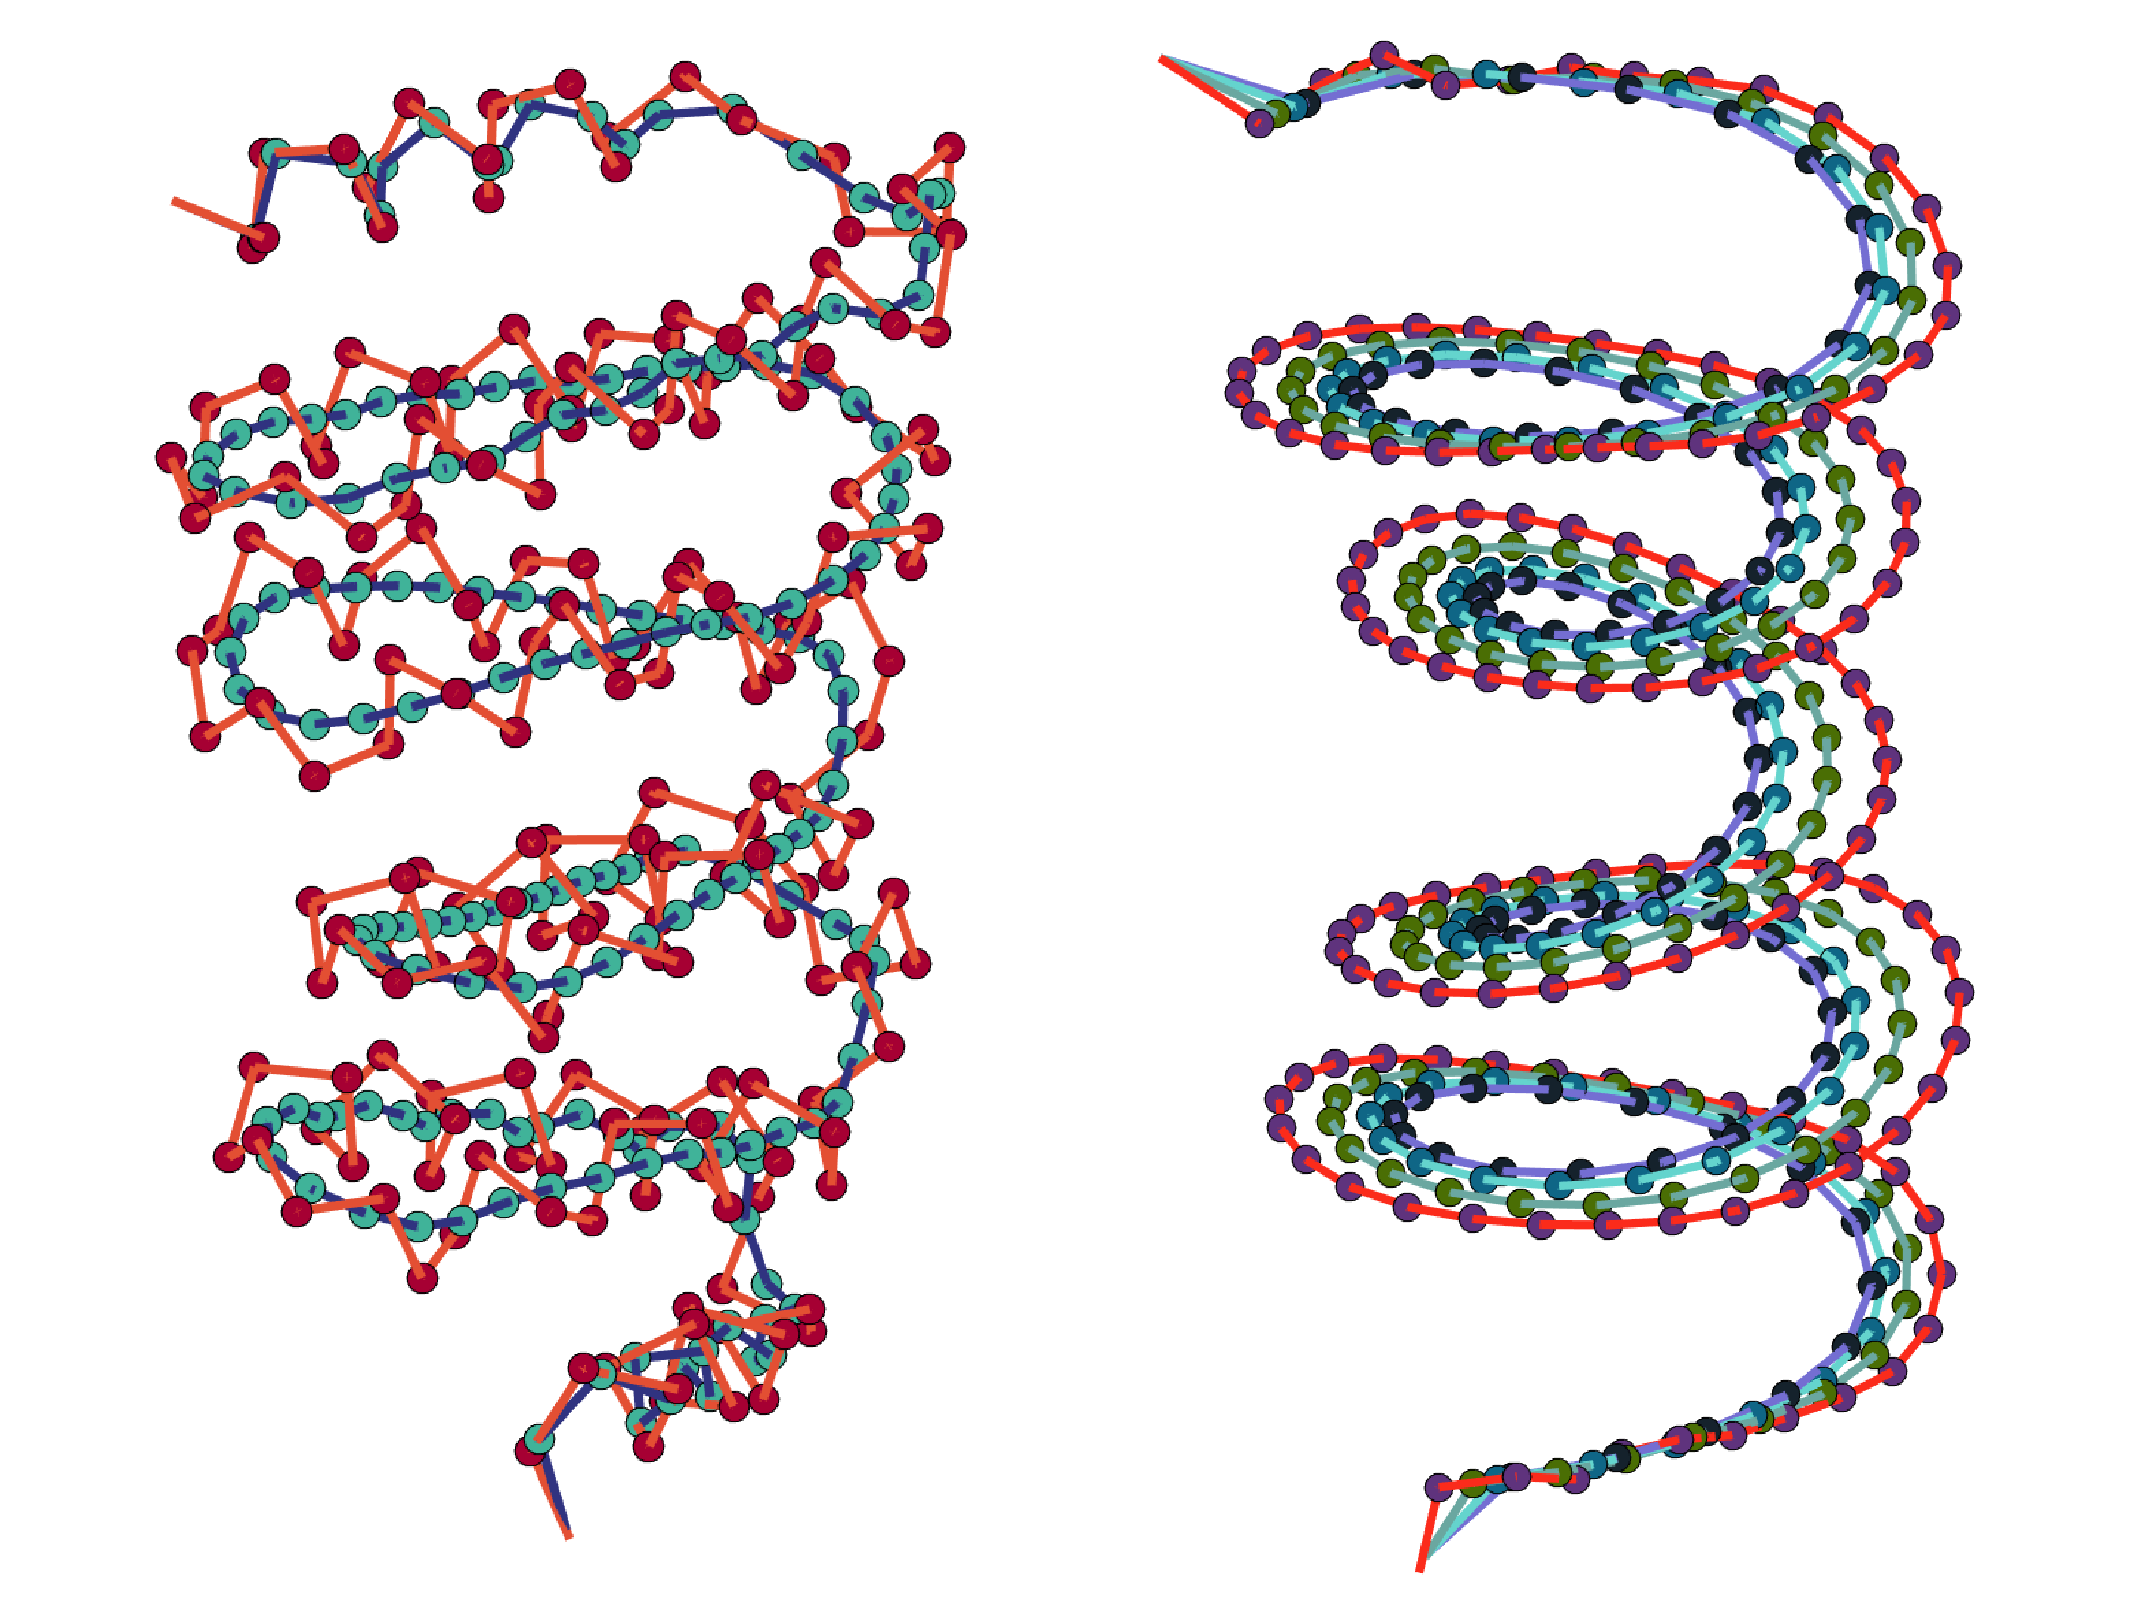
\includegraphics[width=0.7\linewidth]{scaling.pdf}
  	\caption{A subfigure}
	\label{fig:scaling}
\end{figure}
For example, for getting the left figure of Figure \ref{fig:scaling} one should call:\\
\comp{>>showConfiguration('5dn7')} \\
\comp{>>showConfiguration('5dn7', 10)} 

And for the right one:\\
\comp{>>showConfiguration('5dn7', 50)} \\
\comp{>>showConfiguration('5dn7', 80)} \\
\comp{>>showConfiguration('5dn7', 100)} \\
\comp{>>showConfiguration('5dn7', 110)} 

\subsection{Movie}
Function \comp{makeScalingMovie('<polymerName>', <increment>)}  makes avi-file with scaling procedure where each frame is a chain at some step of rescaling procedure. The first frame is the original configuration. Then will be the step with number =  increment. Then $2\cdot$increment,  $3\cdot$increment and so on until only 2 segments left.

If you skip the second argument, then Matlab will record the whole procedure frame by frame.

The same as for the previous function, Matlab will try to open \\\comp{"results/<polymerName>\_configurations.dat"}, so be sure you have it.

\end{homeworkProblem}
%----------------------------------------------------------------------------------------
%	VISUALISATION IN PHYTHON
%----------------------------------------------------------------------------------------

\subsection{Show Configuration}
\begin{homeworkProblem}[Visualization with Python]\label{sec:matlab}
In folder \comp{tools} you can find \comp{PlotterPy} - interactive 3D plotter for \comp{.pca} files.
The plotter is written in \comp{Python 2.7} with using \comp{Matplotlib}.\footnote{If you use MacOS, then you do not need to install anything}. There are two ways how you can run the plotters: from command line or from Python shell.
\subsubsection{From command line}
The program should be run like this:
\begin{lstlisting}
@PlotterPy$@ python <path/to/>plotter.py <path/to/fileName>
 <configuration1> <configuration2> <...>
\end{lstlisting}

For example, if you want to open 5dn7.pca which is stored in folder \comp{results}. And this folder \comp{results} is at the same level as folder \comp{PlotterPy}, then you can run from \comp{PlotterPy} folder:
\begin{lstlisting}
@PlotterPy$@ python ./plotter.py ../results/5dn7.pca
\end{lstlisting}
and see the original configuration, i.e. configuration number 0.

Try:
\begin{lstlisting}
@PlotterPy$@ python ./plotter.py ../results/1abs.pca 50 80 100 110
\end{lstlisting}
to see the corresponding step of rescaling procedure together and get picture similar to \ref{fig:scaling} at the right.

This method is convenient when you want quickly plot configurations. However, if you want to run this program a lot of times, especially if your files are big, we recommend you to go for option two.

\subsubsection{From Python shell}
Running from Python shell will require a bit of work from you, but will same your time in a long run.
First of all we should launch Python:
\begin{lstlisting}
@PlotterPy$@ python
\end{lstlisting}
Then we want to import system library and file with model:
\begin{lstlisting}
@>>>@ import sys
@>>>@ import Polymer
\end{lstlisting}
Now we have to set polymer from file. If we have the same file organization as in the previous section then we do this:
 \begin{lstlisting}
@>>>@ polymer  = Polymer.Polymer('../results/5dn7.pca')
\end{lstlisting}
The next step is to set configurations we want to plot in the same figure.  We want to pass them as arguments. The first argument mast be the name of the program itself:
\begin{lstlisting}
@>>>@ sys.argv = ['plt.py' , '0' ,  '10']
\end{lstlisting}
Now to plot figure similar to \ref{fig:scaling} at the left we execute the plotter:
\begin{lstlisting}
@>>>@ execfile('plt.py')
\end{lstlisting}
If you want to plot some other figure, just repeat two last steps with new values for number of configurations:
\begin{lstlisting}
@>>>@ sys.argv = ['plt.py' , '12' ]
@>>>@ execfile('plt.py')
\end{lstlisting}
It is also very easy to open another file. To finish Python print exit().\\
\hint You can copy-past all the commands from \comp{plt.py}, which you can open with any text editor.
\subsection{Make Gif}

\end{homeworkProblem}
%----------------------------------------------------------------------------------------
%----------------------------------------------------------------------------------------
%	GNUplot
%----------------------------------------------------------------------------------------

\begin{homeworkProblem}[GNUplot]\label{sec:gnuplot}


\end{homeworkProblem}
%----------------------------------------------------------------------------------------

\end{document}
